%% For double-blind review submission, w/o CCS and ACM Reference (max submission space)
%\documentclass[sigplan,10pt,review,anonymous]{acmart}
%\settopmatter{printfolios=false,printccs=false,printacmref=false}
%% For double-blind review submission, w/ CCS and ACM Reference
%\documentclass[sigplan,review,anonymous]{acmart}\settopmatter{printfolios=true}
%% For single-blind review submission, w/o CCS and ACM Reference (max submission space)
%\documentclass[sigplan,review]{acmart}\settopmatter{printfolios=true,printccs=false,printacmref=false}
%% For single-blind review submission, w/ CCS and ACM Reference
%\documentclass[sigplan,review]{acmart}\settopmatter{printfolios=true}
%% For final camera-ready submission, w/ required CCS and ACM Reference
\documentclass[sigplan,nonacm,anonymous]{acmart}\settopmatter{printfolios=false,printccs=false,printacmref=false}

%% Conference information
%% Supplied to authors by publisher for camera-ready submission;
%% use defaults for review submission.
%\acmConference[ARRAY'22]{ACM SIGPLAN Conference on Programming Languages}{June 13, 2022}{San Diego, CA, USA}
%\acmYear{2018}
%\acmISBN{} % \acmISBN{978-x-xxxx-xxxx-x/YY/MM}
%\acmDOI{} % \acmDOI{10.1145/nnnnnnn.nnnnnnn}
%\startPage{1}

%% Copyright information
%% Supplied to authors (based on authors' rights management selection;
%% see authors.acm.org) by publisher for camera-ready submission;
%% use 'none' for review submission.
\setcopyright{none}
%\setcopyright{acmcopyright}
%\setcopyright{acmlicensed}
%\setcopyright{rightsretained}
%\copyrightyear{2018}           %% If different from \acmYear

\usepackage{dsfont}
\usepackage{stmaryrd}
\usepackage{colortbl}
\usepackage{hyperref}


%% Bibliography style
\bibliographystyle{acmart}

\usepackage{dsfont}
\usepackage{stmaryrd}
\usepackage{colortbl}
\usepackage{hyperref}

\usepackage{amsmath}
\DeclareMathOperator*{\argmax}{argmax}
\DeclareMathOperator*{\argmin}{argmin}
\usepackage{amssymb}

\usepackage[dvipsnames, table]{xcolor}
\usepackage{textcomp}

% Packages
\usepackage[pdf]{graphviz}
\usepackage{mathrsfs}

\newcommand*\circled[1]{\tikz[baseline=-0.1cm]{
  \node[shape=circle,draw,inner sep=0.48pt] (char) {\fontsize{7}{12}\textsf{#1}};}}

\DeclareMathAlphabet{\mathcal}{OMS}{cmsy}{m}{n}
\usepackage{cancel}
\newcommand\ccancel[2][red]{\renewcommand\CancelColor{\color{#1}}\cancel{#2}}
\newcommand{\nDownarrow}{\ensuremath{\text{ }\cancel{\Downarrow}\text{ }}}
\usepackage{centernot}

\usepackage{pgfplots, pgfplotstable}
\pgfplotsset{compat=1.7}
\usepgfplotslibrary{fillbetween}
\usetikzlibrary{patterns}
\pgfmathdeclarefunction{gauss}{2}{\pgfmathparse{1/(#2*sqrt(2*pi))*exp(-((x-#1)^2)/(2*#2^2))}}
\pgfmathdeclarefunction{nil}{1}{\pgfmathparse{0.001}}

\usepackage{arydshln}
\usepackage{adjustbox}
\usepackage{enumerate}
\usepackage{enumitem}
\usepackage{tikz-cd}
\usetikzlibrary{calc}
\usepackage{amsfonts}
%\usepackage{prooftrees}
\usepackage{bussproofs}
\renewcommand{\sectionautorefname}{\S}
\renewcommand{\subsectionautorefname}{\S}
\usepackage{float}

\usepackage{tikz-3dplot}
\usetikzlibrary{3d}
\usetikzlibrary{calligraphy}
\newif\ifshowcellnumber
\showcellnumbertrue

\usepackage{algorithm}
\usepackage{algpseudocode}
\usepackage{algorithmicx}
\usepackage{sourcecodepro}
\usepackage{tikz-qtree}
\usepackage{amsthm}
\usepackage{bm}
\usetikzlibrary{bayesnet}
\usetikzlibrary{arrows}
\usepackage{subcaption}
\usetikzlibrary{backgrounds}
\usetikzlibrary{tikzmark}
\usetikzlibrary{hobby}

\usepackage{mwe}

\newcommand{\E}{\mathbb{E}}
\newcommand{\Var}{\mathrm{Var}}
\newcommand{\Cov}{\mathrm{Cov}}

\newcommand{\CompOrder}{\mathcal{O}}
\def\graphspace{\mathbf{G}}
\def\Uniform{\mbox{\rm Uniform}}
\def\Gaussian{\mbox{\rm Gaussian}}
\def\Bernoulli{\mbox{\rm Bernoulli}}
\def\Dirichlet{\mbox{\rm Dirichlet}}

\usepackage{mathtools}% superior to amsmath
\usepackage{tikz}
% Packages
\usepackage{listings}
\DeclareRobustCommand{\hlred}[1]{{\sethlcolor{pink}\hl{#1}}}
\usepackage{fontspec}

\setmonofont[Scale=0.8]{JetBrainsMono}[
  Contextuals={Alternate},
  Path=./font/,
  Extension = .ttf,
  UprightFont=*-Regular,
  BoldFont=*-Bold,
  ItalicFont=*-Italic,
  BoldItalicFont=*-BoldItalic
]

\usepackage[skins,breakable,listings]{tcolorbox}

\lstdefinelanguage{kotlin}{
  comment=[l]{//},
  commentstyle={\color{gray}\ttfamily},
  emph={delegate, filter, firstOrNull, forEach, it, lazy, mapNotNull, println, repeat, assert, with, head, tail, len, return@},
  numberstyle=\noncopyable,
  identifierstyle=\color{black},
  keywords={abstract, actual, as, as?, break, by, class, companion, continue, data, do, dynamic, else, enum, expect, false, final, for, fun, get, if, import, in, infix, interface, internal, is, null, object, open, operator, override, package, private, public, return, sealed, set, super, suspend, this, throw, true, try, catch, typealias, val, var, vararg, when, where, while, tailrec, reified},
  keywordstyle={\bfseries},
  morecomment=[s]{/*}{*/},
  morestring=[b]",
  morestring=[s]{"""*}{*"""},
  ndkeywords={@Deprecated, @JvmField, @JvmName, @JvmOverloads, @JvmStatic, @JvmSynthetic, Array, Byte, Double, Float, Boolean, Int, Integer, Iterable, Long, Runnable, Short, String, int},
  ndkeywordstyle={\bfseries},
  sensitive=true,
  stringstyle={\ttfamily},
  literate={`}{{\char0}}1,
  escapeinside={(*@}{@*)}
}
\lstdefinelanguage{tidy}{
  comment=[l]{//},
  commentstyle={\color{gray}\ttfamily},
  emph={|, ->, ---},
  emphstyle={\color{red}},
  identifierstyle=\color{black},
  keywords={\|, ->, ---},
  otherkeywords={|,->},
  morekeywords={|,->},
  keywordstyle={\color{blue}\bfseries},
  morecomment=[s]{/*}{*/},
  morestring=[b]",
  morestring=[s]{"""*}{*"""},
  ndkeywords={@Deprecated, @JvmField, @JvmName, @JvmOverloads, @JvmStatic, @JvmSynthetic, Array, Byte, Double, Float, Int, Integer, Iterable, Long, Runnable, Short, String},
  ndkeywordstyle={\color{orange}\bfseries},
  sensitive=true,
  stringstyle={\color{green}\ttfamily},
  literate={`}{{\char0}}1
}

%%%%%%%%%%%%%%%%%%%%%%%%%%%%%%%%%%%%%%%%%%%
%
% Color boxes
%
%%%%%%%%%%%%%%%%%%%%%%%%%%%%%%%%%%%%%%%%%%%

\tcbset{
  enhanced jigsaw,
  breakable,
  listing only,
%  boxsep=-1pt,
%  top=-1pt,
  bottom=0.1cm,
  right=0.5cm,
  overlay first={
    \node[black!50] (S) at (frame.south) {\Large\ding{34}};
    \draw[dashed,black!50] (frame.south west) -- (S) -- (frame.south east);
  },
  overlay middle={
    \node[black!50] (S) at (frame.south) {\Large\ding{34}};
    \draw[dashed,black!50] (frame.south west) -- (S) -- (frame.south east);
    \node[black!50] (S) at (frame.north) {\Large\ding{34}};
    \draw[dashed,black!50] (frame.north west) -- (S) -- (frame.north east);
  },
  overlay last={
    \node[black!50] (S) at (frame.north) {\Large\ding{34}};
    \draw[dashed,black!50] (frame.north west) -- (S) -- (frame.north east);
  },
  before={\par\vspace{5pt}},
  after={\par\vspace{\parskip}\noindent}
}

\definecolor{slightgray}{rgb}{0.90, 0.90, 0.90}

\usepackage{soul}
\makeatletter
\def\SOUL@hlpreamble{%
  \setul{}{3.0ex}%
  \let\SOUL@stcolor\SOUL@hlcolor%
  \SOUL@stpreamble%
}
\makeatother

\newcommand{\inline}[1]{%
  \begingroup%
  \sethlcolor{slightgray}%
  \hl{\ttfamily\footnotesize #1}%
  \endgroup
}

\newcommand{\tinline}[1]{%
  \begingroup%
  \sethlcolor{slightgray}%
  \hl{\ttfamily\tiny #1}%
  \endgroup
}

\newtcblisting{halftidyinput}[1][]{%
  left skip=0.7cm,
  left=0.35cm,
  width=6cm,
%  left=-0.01cm,
  top=-0.1cm,
  bottom=-0.35cm,
  listing options={
    language=tidy,
    basicstyle=\ttfamily\small,
%numberstyle=\footnotesize,
    showstringspaces=false,
    tabsize=2,
    breaklines=true,
    numbers=none,
    inputencoding=utf8,
    escapeinside={(*@}{@*)},
    #1
  },
  underlay unbroken and first={%
    \path[draw=none] (interior.north west) rectangle node[white]{
\includegraphics[width=4mm]{../figures/tidyparse_logo.png}} ([xshift=-10mm,yshift=-7mm]interior.north west);
  }
}

\newtcblisting{wholetidyinput}[1][]{%
  left skip=0.7cm,
  left=0.35cm,
  top=0.1cm,
  middle=0mm,
  boxsep=0mm,
  listing options={
    language=tidy,
    basicstyle=\ttfamily\small,
%numberstyle=\footnotesize,
    showstringspaces=false,
    tabsize=2,
    breaklines=true,
    numbers=none,
    inputencoding=utf8,
    escapeinside={(*@}{@*)},
    #1
  },
  underlay unbroken and first={%
      \path[draw=none] (interior.north west) rectangle node[white]{
\includegraphics[width=4mm]{../figures/tidyparse_logo.png}} ([xshift=-10mm,yshift=-9mm]interior.north west);
  }
}

\definecolor{A}{RGB}{6,150,104}
\definecolor{B}{RGB}{196,74,137}
\definecolor{C}{RGB}{117,237,133}
\definecolor{D}{RGB}{246,46,243}
\definecolor{E}{RGB}{89,162,12}
\definecolor{F}{RGB}{113,12,158}
\definecolor{G}{RGB}{191,205,142}
\definecolor{H}{RGB}{51,58,158}
\definecolor{I}{RGB}{244,212,3}
\definecolor{J}{RGB}{37,36,249}
\definecolor{K}{RGB}{253,165,71}
\definecolor{L}{RGB}{27,81,29}
\colorlet{LA}{A!30}
\colorlet{LB}{B!30}
\colorlet{LC}{C!30}
\colorlet{LD}{D!30}
\colorlet{LE}{E!30}
\colorlet{LF}{F!30}
\colorlet{LG}{G!30}
\colorlet{LH}{H!30}
\colorlet{LI}{I!30}
\colorlet{LJ}{J!30}
\colorlet{LK}{K!30}
\colorlet{LL}{L!30}
\newcommand{\hiliA}[1]{%
  \colorbox{LA}{$#1$}}
\newcommand{\hiliB}[1]{%
  \colorbox{LB}{$#1$}}
\newcommand{\hiliC}[1]{%
  \colorbox{LC}{$#1$}}
\newcommand{\hiliD}[1]{%
  \colorbox{LD}{$#1$}}
\newcommand{\hiliE}[1]{%
  \colorbox{LE}{$#1$}}
\newcommand{\hiliF}[1]{%
  \colorbox{LF}{$#1$}}
\newcommand{\hiliG}[1]{%
  \colorbox{LG}{$#1$}}
\newcommand{\hiliH}[1]{%
  \colorbox{LH}{$#1$}}
\newcommand{\hiliI}[1]{%
  \colorbox{LI}{$#1$}}
\newcommand{\hiliJ}[1]{%
  \colorbox{LJ}{$#1$}}
\newcommand{\hiliK}[1]{%
  \colorbox{LK}{$#1$}}
\newcommand{\hiliL}[1]{%
  \colorbox{LL}{$#1$}}
\newcommand{\highlight}[1]{%
  \colorbox{lgray}{$#1$}}
\colorlet{lred}{red!30}
\colorlet{lorange}{orange!30}
\colorlet{lgreen}{green!30}
\colorlet{lgray}{black!15}
\colorlet{dgray}{black!75}
\DeclareRobustCommand{\hlred}[1]{{\sethlcolor{lred}\hl{#1}}}
\DeclareRobustCommand{\hlorange}[1]{{\sethlcolor{lorange}\hl{#1}}}
\DeclareRobustCommand{\hlgreen}[1]{{\sethlcolor{lgreen}\hl{#1}}}
\DeclareRobustCommand{\hlgray}[1]{{\sethlcolor{lgray}\hl{#1}}}
\DeclareRobustCommand{\caret}[1]{{\sethlcolor{dgray}\textcolor{white}{\hl{#1}}}}

\usepackage{url}
\usepackage{qtree}

\usepackage{filecontents}
\usepackage{pstricks-add}
\usepackage{emoji}
\usepackage{alltt}
\usepackage{nicematrix}
\usepackage{graphicx}
\usepackage{ulem}
\usepackage{upquote}
\tikzstyle{every picture}+=[remember picture]
\usepackage{menukeys}
\pgfplotstableread[col sep=comma,]{timings_loc.csv}\loctimings
\pgfplotstableread[col sep=comma,]{timings_unloc.csv}\unloctimings

\makeatletter
\DeclareRobustCommand{\cev}[1]{%
  {\mathpalette\do@cev{#1}}%
}
\newcommand{\do@cev}[2]{%
  \vbox{\offinterlineskip
  \sbox\z@{$\m@th#1 x$}%
  \ialign{##\cr
  \hidewidth\reflectbox{$\m@th#1\vec{}\mkern4mu$}\hidewidth\cr
  \noalign{\kern-\ht\z@}
    $\m@th#1#2$\cr
  }%
  }%
}
\makeatother

\makeatletter
\DeclareRobustCommand{\pder}[1]{%
  \@ifnextchar\bgroup{\@pder{#1}}{\@pder{}{#1}}}
\newcommand{\@pder}[2]{\frac{\partial#1}{\partial#2}}
\makeatother

\newcommand{\shup}{\shortuparrow}
\newcommand{\shri}{\shortrightarrow}
\newcommand{\shur}{\shup\hspace{-5pt}\shri}

\makeatletter
\def\squigglyred{\bgroup \markoverwith{\textcolor{red}{\lower3\p@\hbox{\sixly \char58}}}\ULon}
\makeatother

\makeatletter
\def\squigglyblu{\bgroup \markoverwith{\textcolor{blue}{\lower3\p@\hbox{\sixly \char58}}}\ULon}
\makeatother

\makeatletter
\def\squigglyora{\bgroup \markoverwith{\textcolor{orange}{\lower3\p@\hbox{\sixly \char58}}}\ULon}
\makeatother

\newcommand{\err}[1]{\smash{\squigglyred{#1}{}}}
\newcommand{\erb}[1]{\smash{\squigglyblu{#1}{}}}
\newcommand{\ero}[1]{\smash{\squigglyora{#1}{}}}
\newcommand{\stirlingii}{\genfrac{\{}{\}}{0pt}{}}

%======== Arrows =========
\newcommand{\knightarrow}{
  \tikz{
    \fill (0pt,0pt) circle [radius = 1pt];
    \fill (0pt,6pt) circle [radius = 1pt];
    \fill (6pt,0pt) circle [radius = 1pt];
    \fill (6pt,6pt) circle [radius = 1pt];
    \fill (12pt,0pt) circle [radius = 1pt];
    \fill (12pt,6pt) circle [radius = 1pt];
    \fill (6pt,0pt) circle [radius = 1pt];
    \fill (12pt,0pt) circle [radius = 1pt];
    \draw [-to] (0pt,0pt) -- (12pt,6pt);
  }
}

\newcommand{\kingarrow}{
  \tikz{
    \fill (0pt,0pt) circle [radius = 1pt];
    \fill (6pt,0pt) circle [radius = 1pt];
    \fill (0pt,6pt) circle [radius = 1pt];
    \fill (6pt,6pt) circle [radius = 1pt];
    \draw [-to] (0pt,0pt) -- (6pt,6pt);
    \draw [-to] (0pt,0pt) -- (0pt,6pt);
    \draw [-to] (0pt,0pt) -- (6pt,0pt);
  }
}

\newcommand{\duparrow}{
  \tikz{
    \fill (0pt,0pt) circle [radius = 1pt];
    \fill (0pt,6pt) circle [radius = 1pt];
    \draw [-to] (0pt,0pt) -- (0pt,6pt);
  }
}

\newcommand{\drightarrow}{
  \tikz{
    \fill (0pt,0pt) circle [radius = 1pt];
    \fill (6pt,0pt) circle [radius = 1pt];
    \draw [-to] (0pt,0pt) -- (6pt,0pt);
  }
}

\newcommand{\ddiagarrow}{
  \tikz{
    \fill (0pt,0pt) circle [radius = 1pt];
    \fill (6pt,0pt) circle [radius = 1pt];
    \fill (0pt,6pt) circle [radius = 1pt];
    \fill (6pt,6pt) circle [radius = 1pt];
    \draw [-to] (0pt,0pt) -- (6pt,6pt);
  }
}

\newcommand{\knightkingarrow}{
  \tikz{
    \fill (0pt,0pt) circle [radius = 1pt];
    \fill (0pt,6pt) circle [radius = 1pt];
    \fill (6pt,0pt) circle [radius = 1pt];
    \fill (6pt,6pt) circle [radius = 1pt];
    \fill (12pt,0pt) circle [radius = 1pt];
    \fill (12pt,6pt) circle [radius = 1pt];
    \draw [-to] (0pt,0pt) -- (6pt,6pt);
    \draw [-to] (0pt,0pt) -- (0pt,6pt);
    \draw [-to] (0pt,0pt) -- (6pt,0pt);
    \draw [-to] (0pt,0pt) -- (12pt,6pt);
  }
}

%======== Arrows =========

\usetikzlibrary{decorations.pathreplacing,automata,calc,positioning,matrix,fit,decorations.pathmorphing}

\usepackage{wrapfig}

\newcommand{\mkTrellis}[1]{
  \begin{tikzpicture}
    \def\dx{20pt}
    \def\dy{30pt}
    \newcounter{i}
    \stepcounter{i}
    \node[circle, draw, fill=black!30] (\arabic{i}) at (0,0){};
    \foreach [count=\i] \x in {2,...,#1}{
      \pgfmathsetmacro{\lox}{\x-1}%
      \pgfmathsetmacro{\loxt}{\x-3}%
      \foreach [count=\j] \xx in {-\lox,-\loxt,...,\lox}{
        \pgfmathsetmacro{\jj}{\j-1}%
        \stepcounter{i}
        \pgfmathsetmacro{\kk}{\xx-2}%
        \pgfmathsetmacro{\lbl}{\lox!/(\jj!*(\lox-\jj)!)}
        \ifnum\x<\kk
        \pgfmath\node[circle, draw]  (\arabic{i}) at (\xx*\dx, -\lox*\dy) {};
        \else
        \pgfmath\node[circle, draw, fill=black!30]  (\arabic{i}) at (\xx*\dx, -\lox*\dy) {};
        \fi
      }
    }
    \newcounter{z}
    \newcounter{xn}
    \newcounter{xnn}
    \pgfmathsetmacro{\maxx}{#1 - 1}
    \foreach \x in {1,...,\maxx}{
      \foreach \xx in {1,...,\x}{
        \stepcounter{z}
        \setcounter{xn}{\arabic{z}}
        \addtocounter{xn}{\x}
        \setcounter{xnn}{\arabic{xn}}
        \stepcounter{xnn}
        \draw [<-] (\arabic{z}) -- (\arabic{xn});
        \draw [<-] (\arabic{z}) -- (\arabic{xnn});
      }
    }
  \end{tikzpicture}
}

\newcommand{\dx}{20pt}
\newcommand{\dy}{30pt}
\newcounter{i}
\newcounter{z}
\newcounter{xn}
\newcounter{xnn}
\newcommand{\mkTrellisAppend}[1]{
  \begin{tikzpicture}
    \setcounter{i}{0}
    \setcounter{z}{0}
    \setcounter{xn}{0}
    \setcounter{xnn}{0}
    \stepcounter{i}
    \node[circle, draw] (\arabic{i}) at (0,0){};
    \foreach [count=\i] \x in {2,...,#1}{
      \pgfmathsetmacro{\lox}{\x-1}%
      \pgfmathsetmacro{\loxt}{\x-3}%
      \foreach [count=\j] \xx in {-\lox,-\loxt,...,\lox}{
        \pgfmathsetmacro{\jj}{\j-1}%
        \stepcounter{i}
        \pgfmathsetmacro{\kk}{\xx+2}%
        \pgfmathsetmacro{\lbl}{\lox!/(\jj!*(\lox-\jj)!)}
        \ifnum\x>\kk
        \pgfmath\node[circle, draw, fill=black!30]  (\arabic{i}) at (\xx*\dx, -\lox*\dy) {};
        \else
        \pgfmath\node[circle, draw]  (\arabic{i}) at (\xx*\dx, -\lox*\dy) {};
        \fi
      }
    }
    \pgfmathsetmacro{\maxx}{#1 - 1}
    \foreach \x in {1,...,\maxx}{
      \foreach \xx in {1,...,\x}{
        \stepcounter{z}
        \setcounter{xn}{\arabic{z}}
        \addtocounter{xn}{\x}
        \setcounter{xnn}{\arabic{xn}}
        \stepcounter{xnn}
        \draw [<-] (\arabic{z}) -- (\arabic{xn});
        \draw [<-] (\arabic{z}) -- (\arabic{xnn});
      }
    }
  \end{tikzpicture}
}

\newcommand{\mkTrellisInsert}[1]{
  \begin{tikzpicture}
    \setcounter{i}{0}
    \setcounter{z}{0}
    \setcounter{xn}{0}
    \setcounter{xnn}{0}
    \stepcounter{i}
    \node[circle, draw] (\arabic{i}) at (0,0){};
    \foreach [count=\i] \x in {2,...,#1}{
      \pgfmathsetmacro{\lox}{\x-1}%
      \pgfmathsetmacro{\loxt}{\x-3}%
      \foreach [count=\j] \xx in {-\lox,-\loxt,...,\lox}{
        \pgfmathsetmacro{\jj}{\j-1}%
        \stepcounter{i}
        \pgfmathsetmacro{\mp}{\xx+#1}%
        \pgfmathsetmacro{\mq}{\xx+\x}%
        \pgfmathsetmacro{\lbl}{\lox!/(\jj!*(\lox-\jj)!)}
        \ifnum\x>\mp
        \pgfmath\node[circle, draw, fill=black!30]  (\arabic{i}) at (\xx*\dx, -\lox*\dy) {};
        \else
        \ifnum#1<\mq
        \pgfmath\node[circle, draw, fill=black!30]  (\arabic{i}) at (\xx*\dx, -\lox*\dy) {};
        \else
        \pgfmath\node[circle, draw]  (\arabic{i}) at (\xx*\dx, -\lox*\dy) {};
        \fi
        \fi

      }
    }
    \pgfmathsetmacro{\maxx}{#1 - 1}
    \foreach \x in {1,...,\maxx}{
      \foreach \xx in {1,...,\x}{
        \stepcounter{z}
        \setcounter{xn}{\arabic{z}}
        \addtocounter{xn}{\x}
        \setcounter{xnn}{\arabic{xn}}
        \stepcounter{xnn}
        \draw [<-] (\arabic{z}) -- (\arabic{xn});
        \draw [<-] (\arabic{z}) -- (\arabic{xnn});
      }
    }
  \end{tikzpicture}
}

\usetikzlibrary{automata, positioning, arrows}

\newcommand{\nobarfrac}{\genfrac{}{}{0pt}{}}
\pgfplotstableread[col sep=comma,]{timings_loc.csv}\loctimings
\pgfplotstableread[col sep=comma,]{timings_unloc.csv}\unloctimings
\pgfplotstableread[col sep=comma,]{natural_errors.csv}\naturalerrors
\pgfplotstableread[col sep=comma,]{synthetic_errors.csv}\syntheticerrors

\usepackage[all,pdf]{xy}

\newcommand{\bs}{\blacksquare}
\newcommand{\ws}{\square}
\begin{document}

  \title{Propagation of Syntax Errors in Context-Sensitive\\Languages using the Lifted Brzozowski Derivative}
  \begin{abstract}
    Brzozowski (1964) defines the derivative of a regular language as the suffixes that complete a known prefix. In this work, we establish a Galois connection with Valiant's (1975) fixpoint construction in the context-free setting, and further extend their work into the hierarchy of bounded context-sensitive languages realizable by finite CFL intersection. We show how context-sensitive language recognition can be reduced into a tensor algebra over finite fields, drawing a loose analogy to partial differentiation in Euclidean spaces. In addition to its theoretical contributions, our method has yielded applications to incremental parsing, code completion and program repair. For example, we use it to repair syntax errors and perform sketch-based program synthesis, among other language decision problems.
  \end{abstract}

  \author{Breandan Mark Considine}
  \affiliation{\institution{McGill University}}
  \email{bre@ndan.co}

  \author{Xujie Si}
  \affiliation{\institution{McGill University}}
  \email{xsi@cs.mcgill.ca}

  \maketitle

  \section{Introduction}

  Recall that a CFG is a quadruple consisting of terminals $(\Sigma)$, nonterminals $(V)$, productions $(P\colon V \rightarrow (V \mid \Sigma)^*)$, and a start symbol, $(S)$. It is a well-known fact that every CFG is reducible to \textit{Chomsky Normal Form}, $P'\colon V \rightarrow (V^2 \mid \Sigma)$, in which every production takes one of two forms, either $w \rightarrow xz$, or $w \rightarrow t$, where $w, x, z: V$ and $t: \Sigma$. For example, the CFG, $P:=\{S \rightarrow S S \mid ( S ) \mid ()\}$, corresponds to the CNF:\vspace{-3pt}

  \begin{table}[H]
    \begin{tabular}{llll}
      $P'=\big\{\;S\rightarrow QR \mid SS \mid LR,$ & $L \rightarrow (,$ & $R \rightarrow ),$ & $Q\rightarrow LS\;\big\}$
    \end{tabular}
  \end{table}\vspace{-8pt}

  \noindent Given a CFG, $\mathcal{G}' : \langle \Sigma, V, P, S\rangle$ in CNF, we can construct a recognizer $R: \mathcal{G}' \rightarrow \Sigma^n \rightarrow \mathbb{B}$ for strings $\sigma: \Sigma^n$ as follows. Let $2^V$ be our domain, $0$ be $\varnothing$, $\oplus$ be $\cup$, and $\otimes$ be defined as:\vspace{-10pt}

  \begin{align}
    X \otimes Z := \big\{\;w \mid \langle x, z\rangle \in X \times Z, (w\rightarrow xz) \in P\;\big\}
  \end{align}

  \noindent If we define $\shup\sigma_r \coloneqq \{w \mid (w \rightarrow \sigma_r) \in P\}$, then initialize $M^0_{r+1=c}(\mathcal{G}', e) := \;\shup\sigma_r$ and solve for the fixpoint $M^* = M + M^2$,\vspace{-10pt}

  \begin{align*}
      M^0:=\begin{pNiceMatrix}[nullify-dots,xdots/line-style=loosely dotted]
               \varnothing & \sigma_1^\shup & \varnothing & \Cdots & \varnothing \\
               \Vdots      & \Ddots         & \Ddots      & \Ddots & \Vdots\\
                           &                &             &        & \varnothing\\
                           &                &             &        & \sigma_n^\shup \\
               \varnothing & \Cdots         &             &        & \varnothing
      \end{pNiceMatrix} &\Rightarrow M^* =
      \begin{pNiceMatrix}[nullify-dots,xdots/line-style=loosely dotted]
        \varnothing & \sigma_1^\shup & \Lambda & \Cdots & \Lambda^*_\sigma\\
        \Vdots      & \Ddots         & \Ddots  & \Ddots & \Vdots\\
                    &                &         &        & \Lambda\\
                    &                &         &        & \sigma_n^\shup \\
        \varnothing & \Cdots         &         &        & \varnothing
      \end{pNiceMatrix}
  \end{align*}

  \noindent we obtain the recognizer, $R(\mathcal{G}', \sigma) := S \in \Lambda^*_\sigma? \Leftrightarrow \sigma \in \mathcal{L}(\mathcal{G})?$

  \noindent Full details of the bisimilarity between parsing and matrix multiplication can be found in Valiant~\cite{valiant1975general} and Lee~\cite{lee2002fast}, who shows its time complexity to be $\mathcal{O}(n^\omega)$ where $\omega$ is the least matrix multiplication upper bound (currently, $\omega < 2.77$).

  \section{Method}

  Note that $\bigoplus_{c = 1}^n M_{r,c} \otimes M_{c,r}$ has cardinality bounded by $|V|$ and is thus representable as a fixed-length vector using the characteristic function, $\mathds{1}$. In particular, $\oplus, \otimes$ are redefined as $\boxplus, \boxtimes$ over bitvectors so the following diagram commutes,\footnote{Hereinafter, we use gray highlighting to distinguish between expressions containing only \highlight{\text{constants}} from those which may contain free variables.}

  \begin{figure}[H]
  \adjustbox{scale=0.62,center}{%
  \[\begin{tikzcd}[row sep=large, column sep=huge]
   \langle\mathcal{G}', \highlight{\Sigma}^{n-1}\rangle \arrow[leftrightarrow, drrr, shorten=-1mm] & & [-135pt] & \vspace{20pt}\text{Set} \arrow[d, phantom] & \text{Bit} \arrow[d, phantom] & [-90pt] & \langle\mathcal{G}', \Sigma^{n-1}\rangle \arrow[drr, shorten=-2mm] & [-90pt] & \text{SAT} \arrow[d, phantom]\\[-30pt]
   \text{Rubix}  \arrow[rr, phantom] & & [-135pt] & M \times M \arrow[r, "\mathds{1}^{2^{n\times n}}", labels=above] \arrow[d, "\hspace{-13pt}\bigoplus\:\bigotimes"] & \mathbb{Z}_2^{|V|^{n\times n}} \times \mathbb{Z}_2^{|V|^{n\times n}} \arrow[d, "\hspace{-13.4pt}\highlight{+}\:\highlight{*}"] \arrow[l, "\mathds{1}^{-2^{n\times n}}", labels=below] \arrow[rrrr, rightarrowtail, "\varphi^{2^{n\times n}}", labels=above] & [-90pt] & & [-90pt] & \mathcal{M} \times \mathcal{M} \arrow[llll, rightharpoonup, shorten=1mm, "\varphi^{-2^{n\times n}}", labels=below] \arrow[d, "\hspace{-9pt}+\:\:\:*"] \\
   \text{Matrix} \arrow[rr, phantom] & & [-135pt] & 2^V \times 2^V \arrow[r, "\mathds{1}^{2}", labels=above] \arrow[d, "\hspace{-9pt}\oplus\:\otimes"] & \mathbb{Z}_2^{|V|} \times \mathbb{Z}_2^{|V|} \arrow[d, "\hspace{-15.8pt}\highlight{\boxplus}\:\highlight{\boxtimes}"] \arrow[l, "\mathds{1}^{-2}", labels=below] \arrow[rrrr, rightarrowtail, "\varphi^2", labels=above] & [-90pt] & & [-90pt] & \mathcal{V} \times \mathcal{V} \arrow[llll, rightharpoonup, shorten=1mm, "\varphi^{-2}", labels=below] \arrow[d, "\hspace{-9.5pt}\boxplus\:\boxtimes"] \arrow[u] \\
   \text{Vector} \arrow[rr, phantom] & & [-135pt] & 2^V \arrow[r, "\mathds{1}", labels=above] & \mathbb{Z}_2^{|V|} \arrow[l, "\mathds{1}^{-1}", labels=below] \arrow[rrrr, rightarrowtail, "\varphi", labels=above] & [-90pt] & & [-90pt] & \mathcal{V} \arrow[llll, rightharpoonup, shorten=1mm, "\varphi^{-1}", labels=below] \arrow[u]
  \end{tikzcd}\]
  }
  \end{figure}

%\noindent The compactness of this representation can be improved via a combinatorial number system without loss of generality, although $\mathds{1}$ is a convenient encoding for SAT.

%  \noindent This construction can be lifted into the domain of bitvector variables, producing an algebraic expression for each scalar inhabitant of the northeasternmost bitvector $\mathcal{T}$, whose solutions correspond to valid parse forests for an incomplete string on the superdiagonal.
  \noindent where $\mathcal{V}$ is a function $\mathbb{Z}_2^{|V|}\rightarrow\mathbb{Z}_2$. Note that while always possible to encode $\mathbb{Z}_2^{|V|} \rightarrow \mathcal{V}$ using the identity function, $\varphi^{-1}$ may not exist, as an arbitrary $\mathcal{V}$ might take on zero, one, or in general, multiple values in $\mathbb{Z}_2^{|V|}$. Although holes may occur anywhere, let us consider two cases in which $\Sigma^+$ is strictly left- or right-constrained, i.e., $\highlight{x}z, x\highlight{z}: \Sigma^{|x|+|z|}$.

  Valiant's $\otimes$ operator, which yields the set of productions unifying known factors in a binary CFG, naturally implies the existence of a left- and right-quotient, which yield the set of nonterminals that may appear the right or left side of a known factor and its corresponding root. In other words, a known factor not only implicates subsequent expressions that can be derived from it, but also adjacent factors that may be composed with it to form a given derivation.

  \begin{table}[H]
    \adjustbox{scale=0.92,center}{%
    \begin{tabular}{cccc}
      Left Quotient &&& Right Quotient \\\\
      $\frac{\partial f}{\partial \cev{x}} = \big\{\;w \mid (w \rightarrow x z)\in P\;\big\}$ &&&
      $\frac{\partial f}{\partial \vec{z}} = \big\{\;x \mid (w \rightarrow x z)\in P\;\big\}$ \\\\
      \begin{tabular}{|c|c|}
        \hline
        \cellcolor{black!15}\hspace{-0.5mm}$x$\hspace{-0.5mm} & \cellcolor{black!15}\hspace{-0.95mm}$w$\hspace{-0.95mm} \\ \hline
        \multicolumn{1}{c|}{~} & \hspace{-0.95mm}$z$\hspace{-0.95mm} \\
        \cline{2-2}
      \end{tabular} &&&
      \begin{tabular}{|c|c|}
        \hline
        \hspace{-0.5mm}$x$\hspace{-0.5mm} & \cellcolor{black!15}\hspace{-0.95mm}$w$\hspace{-0.95mm} \\ \hline
        \multicolumn{1}{c|}{~} & \cellcolor{black!15}\hspace{-0.95mm}$z$\hspace{-0.95mm} \\
        \cline{2-2}
      \end{tabular}
    \end{tabular}
    }
  \end{table}

  \noindent The left quotient coincides with the derivative operator first proposed by Brzozowski~\cite{brzozowski1964derivatives} and Antimirov~\cite{antimirov1996partial} over regular languages, lifted into the context-free setting (our work). When the root and LHS are fixed, e.g., $\frac{\partial S}{\partial \cev{x}}: (\cev{V} \rightarrow S) \rightarrow \vec{\mathcal{V}}$ returns the set of admissible nonterminals to the RHS. One may also define a gradient operator, $\cev{\nabla} S: (\cev{\mathcal{V}} \rightarrow S) \rightarrow \vec{\mathcal{V}}$, which simultaneously tracks the partials with respect to a set of multiple LHS nonterminals produced by a fixed root.

%  These operators in the context-free setting respect linearity. The $\oplus$ case is trivial. For $\otimes$, let us consider the left quotient. Its symmetric case is left as an exercise for the reader:
%
%  $\frac{\partial}{\partial x}(f\otimes g) = \frac{\partial f}{\partial x}\otimes g \oplus f\otimes\frac{\partial g}{\partial x}$
%
%  TODO: prove the product rule holds for CFG reachability.

%  If the root itself is unknown, we can define an operator, $\mathcal{H}_{\mathcal{W}\subseteq\mathcal{V}}: (\cev{\mathcal{V}}\times\vec{\mathcal{V}}\times\mathcal{W}) \rightarrow (\vec{\mathcal{V}}\times\vec{\mathcal{V}}\rightarrow\mathcal{W})$, which tracks second-order partial derivatives for all roots in $\mathcal{W}$. Unlike differential calculus on smooth manifolds, partials in this calculus do not necessarily commute depending on the CFG.

  \definecolor{R}{RGB}{202,65,55}
  \definecolor{G}{RGB}{151,216,56}
  \definecolor{W}{RGB}{255,255,255}
  \definecolor{X}{RGB}{65,65,65}

  \newcommand{\TikZRubikFaceLeft}[9]{\def\myarrayL{#1,#2,#3,#4,#5,#6,#7,#8,#9}}
  \newcommand{\TikZRubikFaceRight}[9]{\def\myarrayR{#1,#2,#3,#4,#5,#6,#7,#8,#9}}
  \newcommand{\TikZRubikFaceTop}[9]{\def\myarrayT{#1,#2,#3,#4,#5,#6,#7,#8,#9}}
  \newcommand{\BuildArray}{\foreach \X [count=\Y] in \myarrayL%
  {\ifnum\Y=1%
  \xdef\myarray{"\X"}%
  \else%
  \xdef\myarray{\myarray,"\X"}%
  \fi}%
  \foreach \X in \myarrayR%
  {\xdef\myarray{\myarray,"\X"}}%
  \foreach \X in \myarrayT%
  {\xdef\myarray{\myarray,"\X"}}%
  \xdef\myarray{{\myarray}}%
  }
  \TikZRubikFaceLeft
  {LA}{W}{W}
  {W}{LB}{LC}
  {LD}{W}{W}
  \TikZRubikFaceRight
  {W}{LK}{W}
  {LC}{W}{LG}
  {W}{LH}{W}
  \TikZRubikFaceTop
  {LA}{W}{LI}
  {W}{W}{LJ}
  {W}{LK}{W}
  \BuildArray
  \pgfmathsetmacro\radius{0.1}
  \tdplotsetmaincoords{55}{135}

  \showcellnumberfalse

  \bgroup
  \newcommand\ddd{\Ddots}
  \newcommand\vdd{\Vdots}
  \newcommand\cdd{\Cdots}
  \newcommand\lds{\ldots}
  \newcommand\vno{\varnothing}
  \newcommand{\ts}[1]{\textsuperscript{#1}}
  \newcommand\non{1\ts{st}}
  \newcommand\ntw{2\ts{nd}}
  \newcommand\nth{3\ts{rd}}
  \newcommand\nfo{4\ts{th}}
  \newcommand\nfi{5\ts{th}}
  \newcommand\nsi{6\ts{th}}
  \newcommand\nse{7\ts{th}}
  \newcommand{\vs}[1]{\shup\sigma_{#1}}
  \newcommand\rcr{\rowcolor{black!15}}
  \newcommand\rcw{\rowcolor{white}}
  \newcommand\pcd{\cdot}
  \newcommand\pcp{\phantom\cdot}
  \newcommand\ppp{\phantom{\nse}}

  \begin{figure}
    \[
    \begin{align*}
      o &\rightarrow \hiliD{so} \mid \hiliC{rs} \mid \hiliB{rr}\hspace{0.5pt} \mid \hiliA{oo}\\
      r &\rightarrow \hiliE{so} \mid \hiliH{ss}\hspace{0.4pt}\mid \hiliF{rr}\hspace{0.5pt} \mid \hiliK{os}\\
      s &\rightarrow \hiliL{so} \mid \hiliG{rs} \mid \hiliJ{or} \mid \hiliI{oo}
    \end{align*} \phantom{=} \mathcal{H}_{\{o\}} = \begin{pmatrix}
          \hiliA{\pder{^2 o}{\cev{o}\partial\vec{o}}} & \pder{^2 o}{\cev{o}\partial\vec{r}} & \pder{^2 o}{\cev{o}\partial\vec{s}}\\
          \pder{^2 o}{\cev{r}\partial\vec{o}} & \hiliB{\pder{^2 o}{\cev{r}\partial\vec{r}}} & \hiliC{\pder{^2 o}{\cev{r}\partial\vec{s}}}\\
          \hiliD{\pder{^2 o}{\cev{s}\partial\vec{o}}} & \pder{^2 o}{\cev{s}\partial\vec{r}} & \pder{^2 o}{\cev{s}\partial\vec{s}}
        \end{pmatrix}
%    \mathcal{J} = \begin{pmatrix}
%       \pder{o}{o} & \pder{o}{r} & \pder{o}{s}\\
%       \pder{r}{o} & \pder{r}{r} & \pder{r}{s}\\
%       \pder{s}{o} & \pder{s}{r} & \pder{s}{s}
%    \end{pmatrix}
    \]
    \hspace{-0.5cm}\begin{minipage}[l]{4.3cm}
    \scalebox{0.8}{\begin{tikzpicture}
      \clip (-3,-2.5) rectangle (3,2.5);
      \begin{scope}[tdplot_main_coords]
        \filldraw [canvas is yz plane at x=1.5] (-1.5,-1.5) rectangle (1.5,1.5);
        \filldraw [canvas is xz plane at y=1.5] (-1.5,-1.5) rectangle (1.5,1.5);
        \filldraw [canvas is yx plane at z=1.5] (-1.5,-1.5) rectangle (1.5,1.5);
        \foreach \X [count=\XX starting from 0] in {-1.5,-0.5,0.5}{
          \foreach \Y [count=\YY starting from 0] in {-1.5,-0.5,0.5}{
            \pgfmathtruncatemacro{\Z}{\XX+3*(2-\YY)}
            \pgfmathsetmacro{\mycolor}{\myarray[\Z]}
            \draw [thick,canvas is yz plane at x=1.5,shift={(\X,\Y)},fill=\mycolor] (0.5,0) -- ({1-\radius},0) arc (-90:0:\radius) -- (1,{1-\radius}) arc (0:90:\radius) -- (\radius,1) arc (90:180:\radius) -- (0,\radius) arc (180:270:\radius) -- cycle;
            \ifshowcellnumber
            \node[canvas is yz plane at x=1.5,shift={(\X+0.5,\Y+0.5)}] {\Z};
            \fi
            \pgfmathtruncatemacro{\Z}{2-\XX+3*(2-\YY)+9}
            \pgfmathsetmacro{\mycolor}{\myarray[\Z]}
            \draw [thick,canvas is xz plane at y=1.5,shift={(\X,\Y)},fill=\mycolor] (0.5,0) -- ({1-\radius},0) arc (-90:0:\radius) -- (1,{1-\radius}) arc (0:90:\radius) -- (\radius,1) arc (90:180:\radius) -- (0,\radius) arc (180:270:\radius) -- cycle;
            \ifshowcellnumber
            \node[canvas is xz plane at y=1.5,shift={(\X+0.5,\Y+0.5)},xscale=-1] {\Z};
            \fi
            \pgfmathtruncatemacro{\Z}{2-\YY+3*\XX+18}
            \pgfmathsetmacro{\mycolor}{\myarray[\Z]}
            \draw [thick,canvas is yx plane at z=1.5,shift={(\X,\Y)},fill=\mycolor] (0.5,0) -- ({1-\radius},0) arc (-90:0:\radius) -- (1,{1-\radius}) arc (0:90:\radius) -- (\radius,1) arc (90:180:\radius) -- (0,\radius) arc (180:270:\radius) -- cycle;
            \ifshowcellnumber
            \node[canvas is yx plane at z=1.5,shift={(\X+0.5,\Y+0.5)},xscale=-1,rotate=-90] {\Z};
            \fi
          }
        }
        \draw [decorate,decoration={calligraphic brace,amplitude=10pt,mirror},yshift=0pt, line width=1.25pt]
        (3,0) -- (3,3) node [black,midway,xshift=-8pt, yshift=-14pt] {\footnotesize $V_x$};
        \draw [decorate,decoration={calligraphic brace,amplitude=10pt},yshift=0pt, line width=1.25pt]
        (3,0) -- (0,-3) node [black,midway,xshift=-16pt, yshift=0pt] {\footnotesize $V_y$};
        \draw [decorate,decoration={calligraphic brace,amplitude=10pt},yshift=0pt, line width=1.25pt]
        (0,-3) -- (-3,-3) node [black,midway,xshift=-8pt, yshift=14pt] {\footnotesize $V_w$};
      \end{scope}
    \end{tikzpicture}}
    \end{minipage}
    \begin{minipage}[c]{3.5cm}
      \begin{align*}
        \mathcal{H}_{\{r\}} = & \begin{pmatrix}
           \pder{^2 r}{\cev{o}\partial\vec{o}} & \pder{^2 r}{\cev{o}\partial\vec{r}} & \hiliK{\pder{^2 r}{\cev{o}\partial\vec{s}}}\\
           \pder{^2 r}{\cev{r}\partial\vec{o}} & \hiliF{\pder{^2 r}{\cev{r}\partial\vec{r}}} & \pder{^2 r}{\cev{r}\partial\vec{s}}\\
           \hiliE{\pder{^2 r}{\cev{s}\partial\vec{o}}} & \pder{^2 r}{\cev{s}\partial\vec{r}} & \hiliH{\pder{^2 r}{\cev{s}\partial\vec{s}}}
        \end{pmatrix}
      \end{align*}
        \begin{align*}
        \mathcal{H}_{\{s\}} = & \begin{pmatrix}
           \hiliI{\pder{^2 s}{\cev{o}\partial\vec{o}}} & \hiliJ{\pder{^2 s}{\cev{o}\partial\vec{r}}} & \pder{^2 s}{\cev{o}\partial\vec{s}}\\
           \pder{^2 s}{\cev{r}\partial\vec{o}} & \pder{^2 s}{\cev{r}\partial\vec{r}} & \hiliG{\pder{^2 s}{\cev{r}\partial\vec{s}}}\\
           \hiliL{\pder{^2 s}{\cev{s}\partial\vec{o}}} & \pder{^2 s}{\cev{s}\partial\vec{r}} & \pder{^2 s}{\cev{s}\partial\vec{s}}
        \end{pmatrix}
      \end{align*}
    \end{minipage}
    \caption{CFGs are witnessed by a rank-3 binary tensor, whose nonzero entries indicate CNF productions. Derivatives in this setting effectively condition the parse tensor. By backpropagating $\mathcal{H}$ across upper-triangular entries of $\mathcal{M}^*$, we constrain the superposition of admissible parse forests.}
  \end{figure}

%  \noindent By allowing the matrix $\mathcal{M}^*$ to contain bitvector variables representing holes in $\sigma$, we obtain a set of multilinear equations whose solutions exactly correspond to the set of admissible repairs and their corresponding parse forests. Specifically, the repairs coincide with holes in the superdiagonal $\mathcal{M}^*_{r+1 = c}$, and the parse forests occur along upper-triangular entries $\mathcal{M}^*_{r + 1 < c}$. In the follow case, $\mathcal{M}^*$ is left-constrained, although the holes may (in general) appear anywhere in $\sigma$:
%
%%We precompute the shadow of fully-resolved substrings before feeding it to the SAT solver. If the substring is known, we can simply compute this directly outside the SAT solver. Shaded regions are bitvector literals and light regions correspond to bitvector variables.
%
%%We illustrate this fact in \S\ref{sec:error}:
%%
%%\begin{figure}[H]
%%    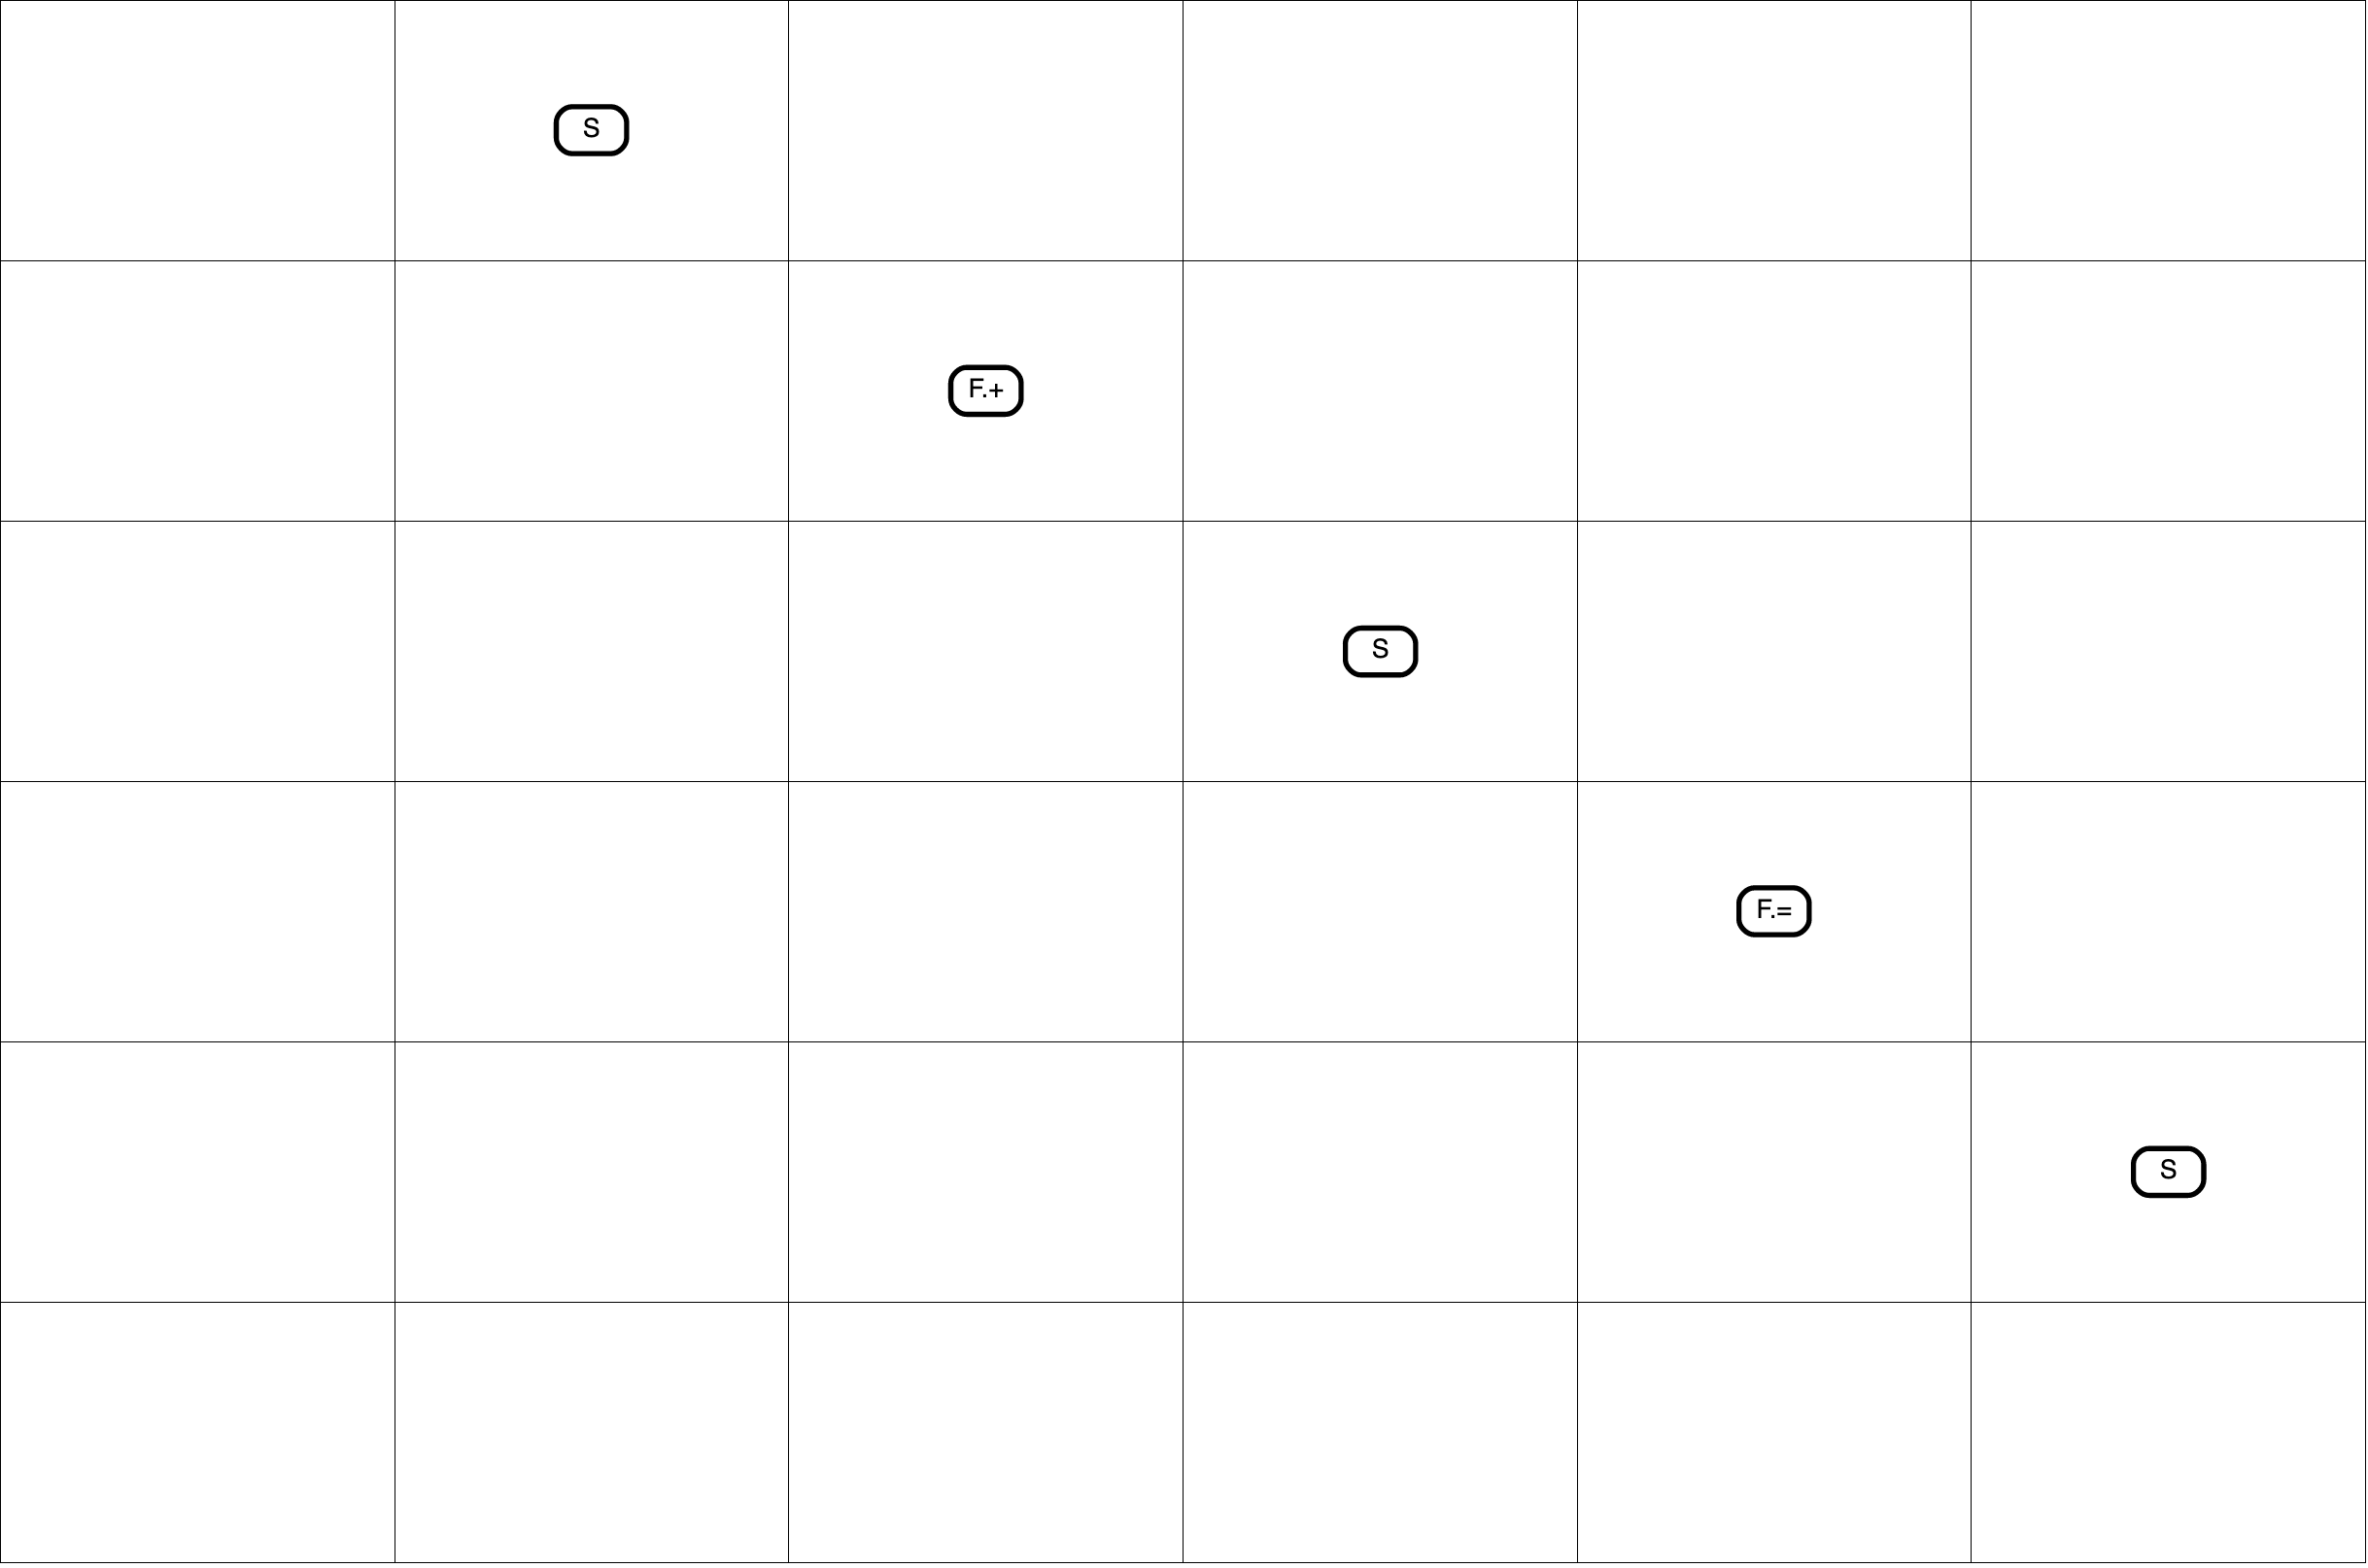
\includegraphics[width=2cm]{../figures/parse1.png}
%%    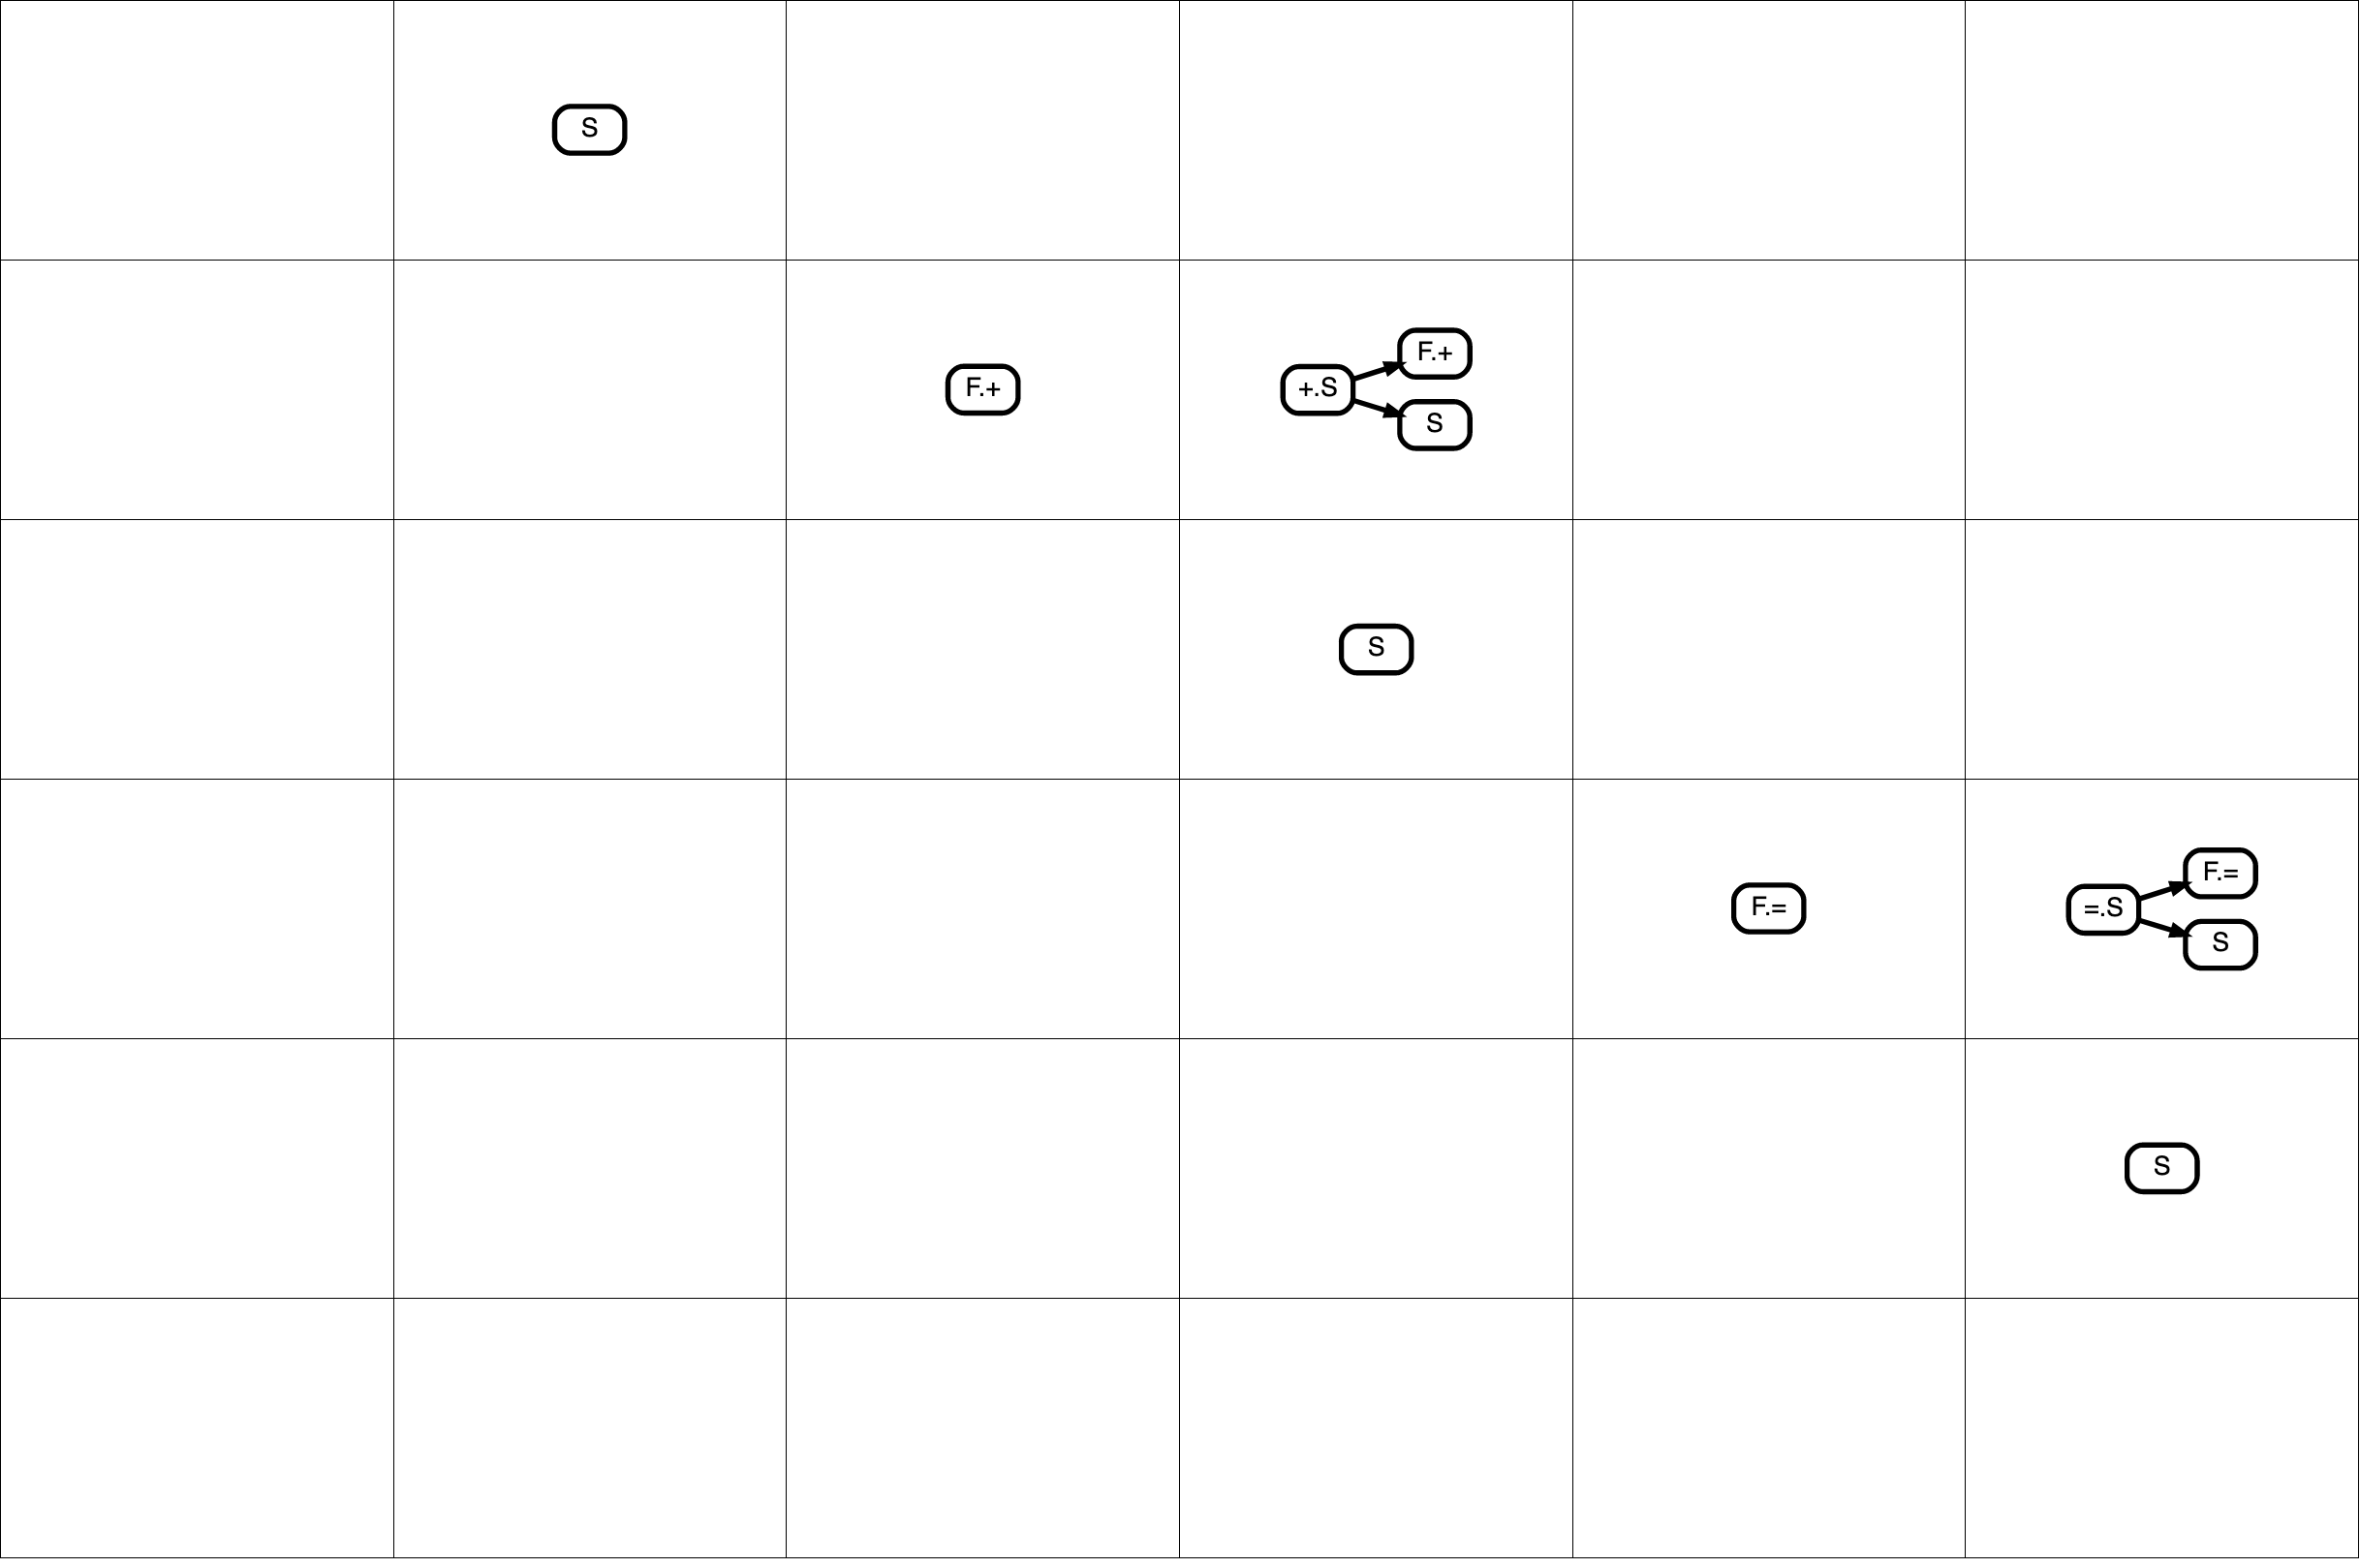
\includegraphics[width=2cm]{../figures/parse2.png}
%%    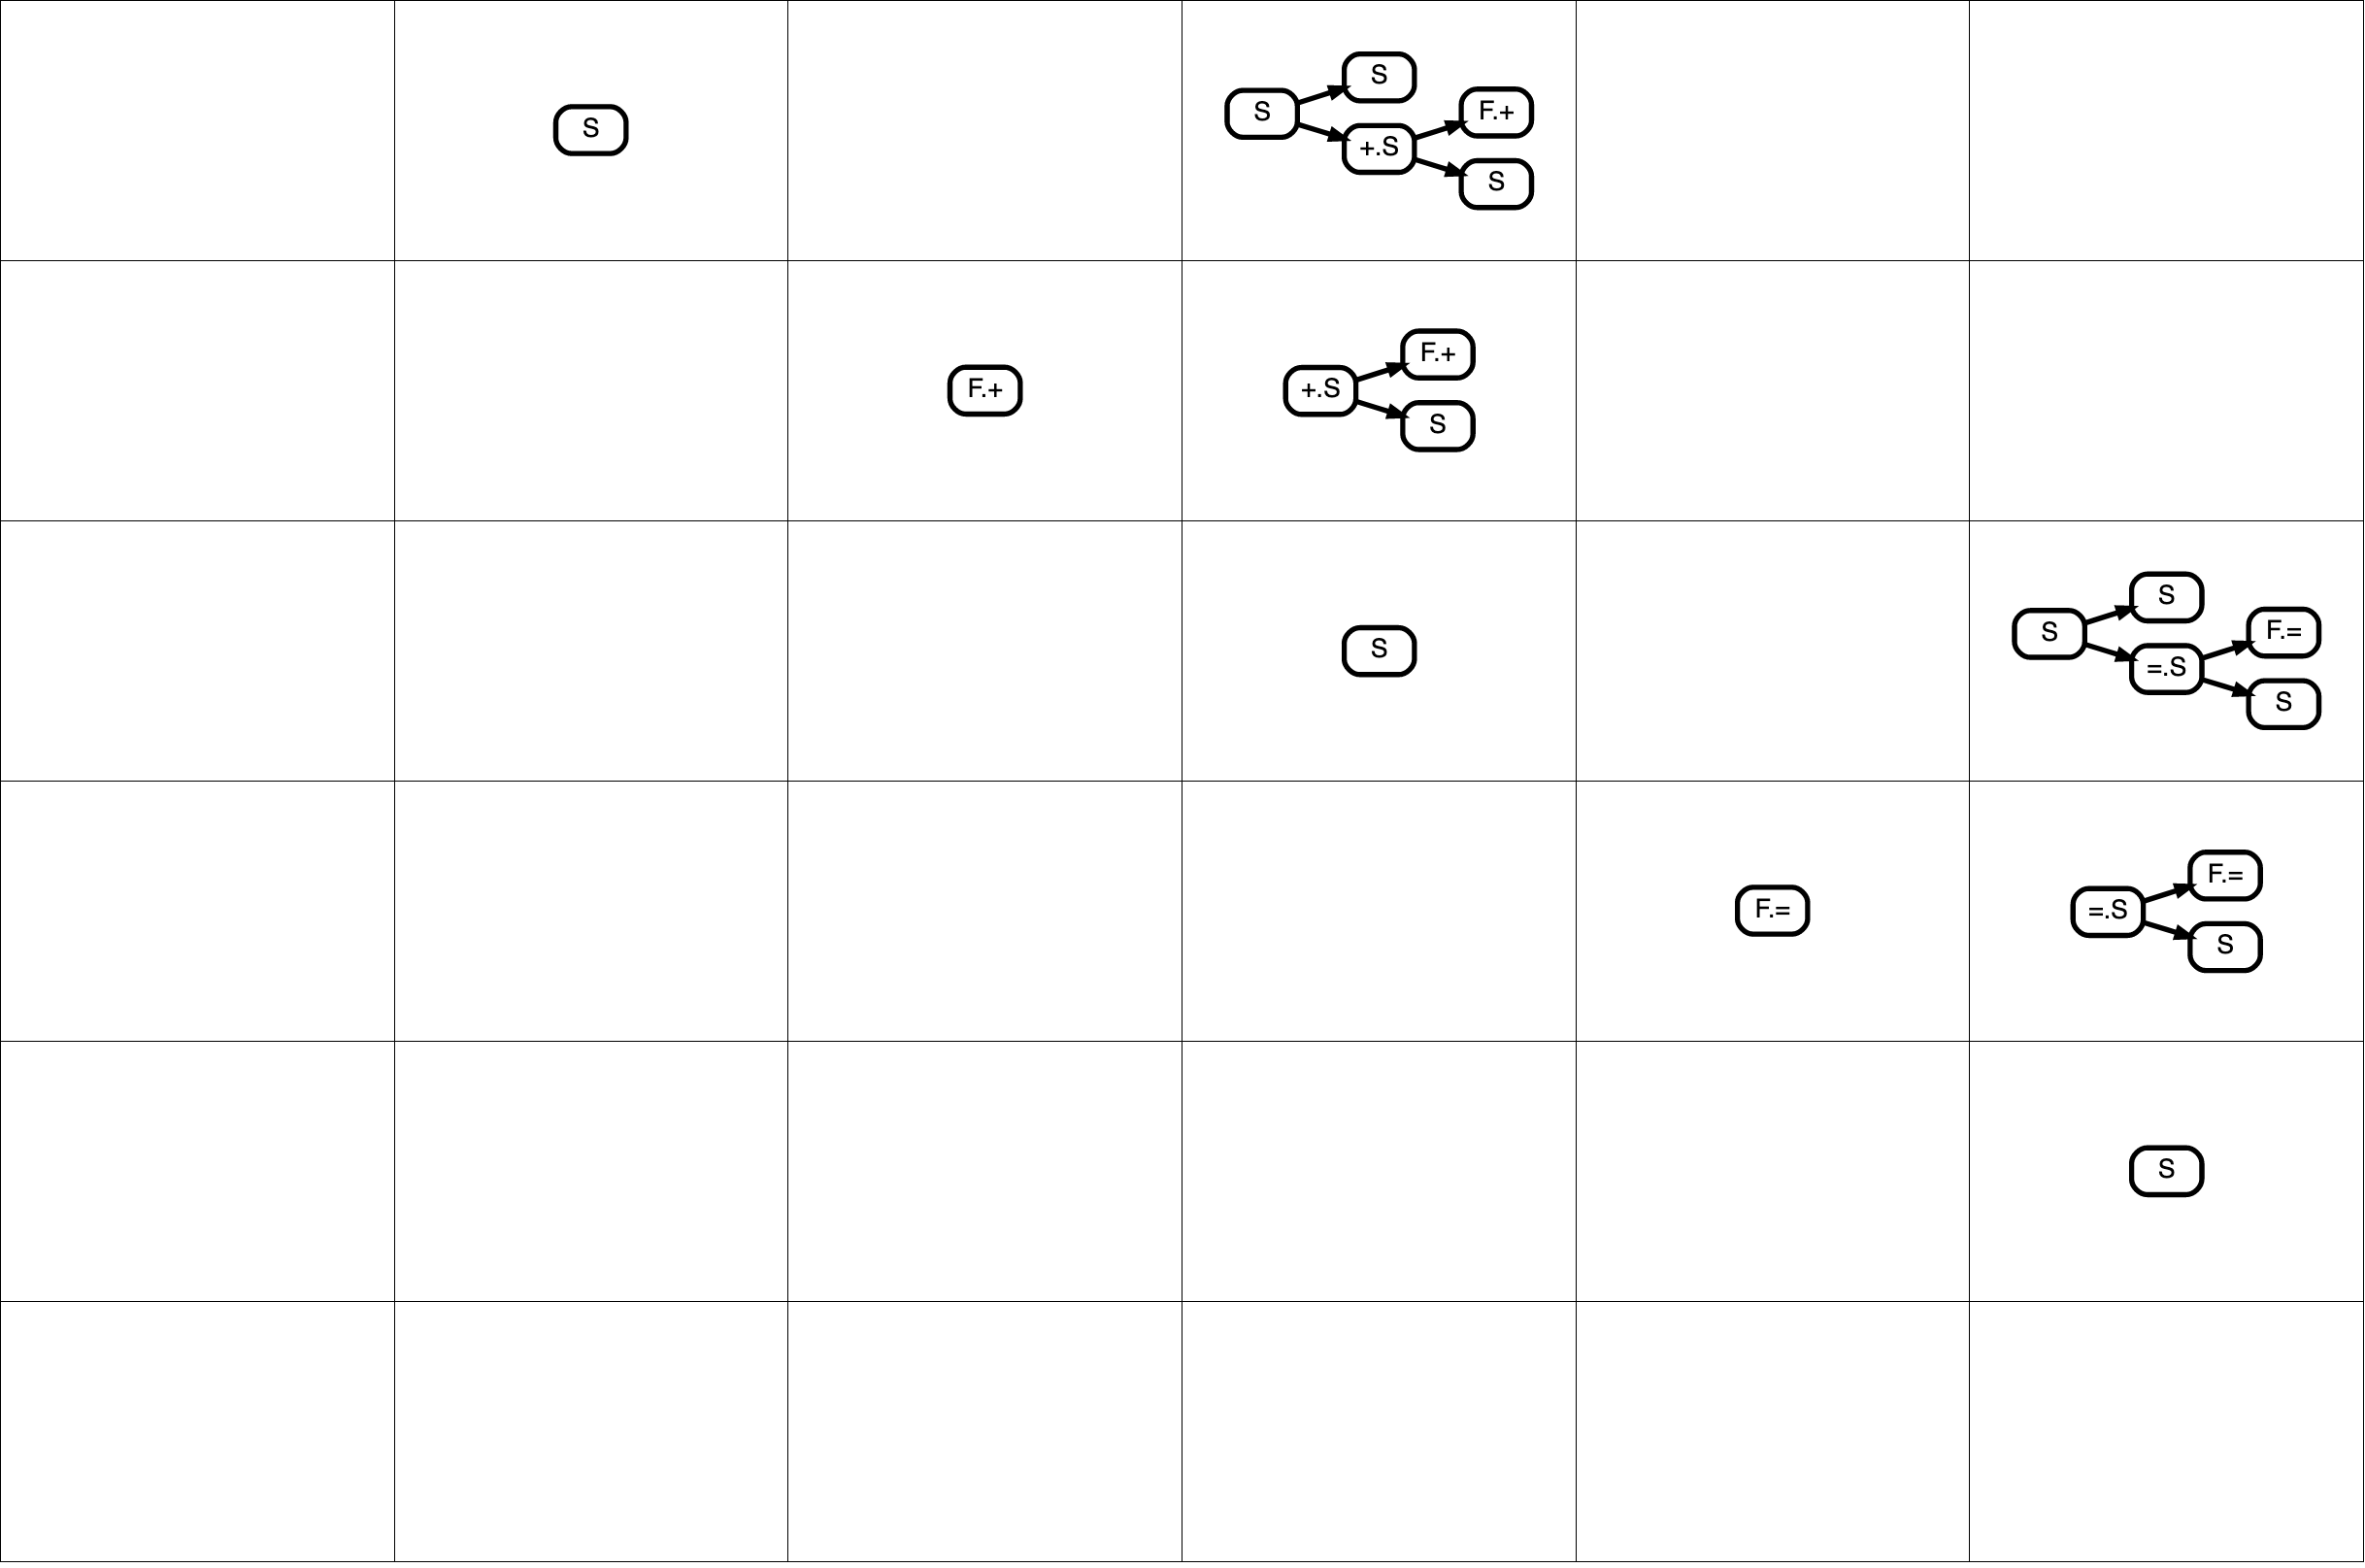
\includegraphics[width=2cm]{../figures/parse3.png}
%%    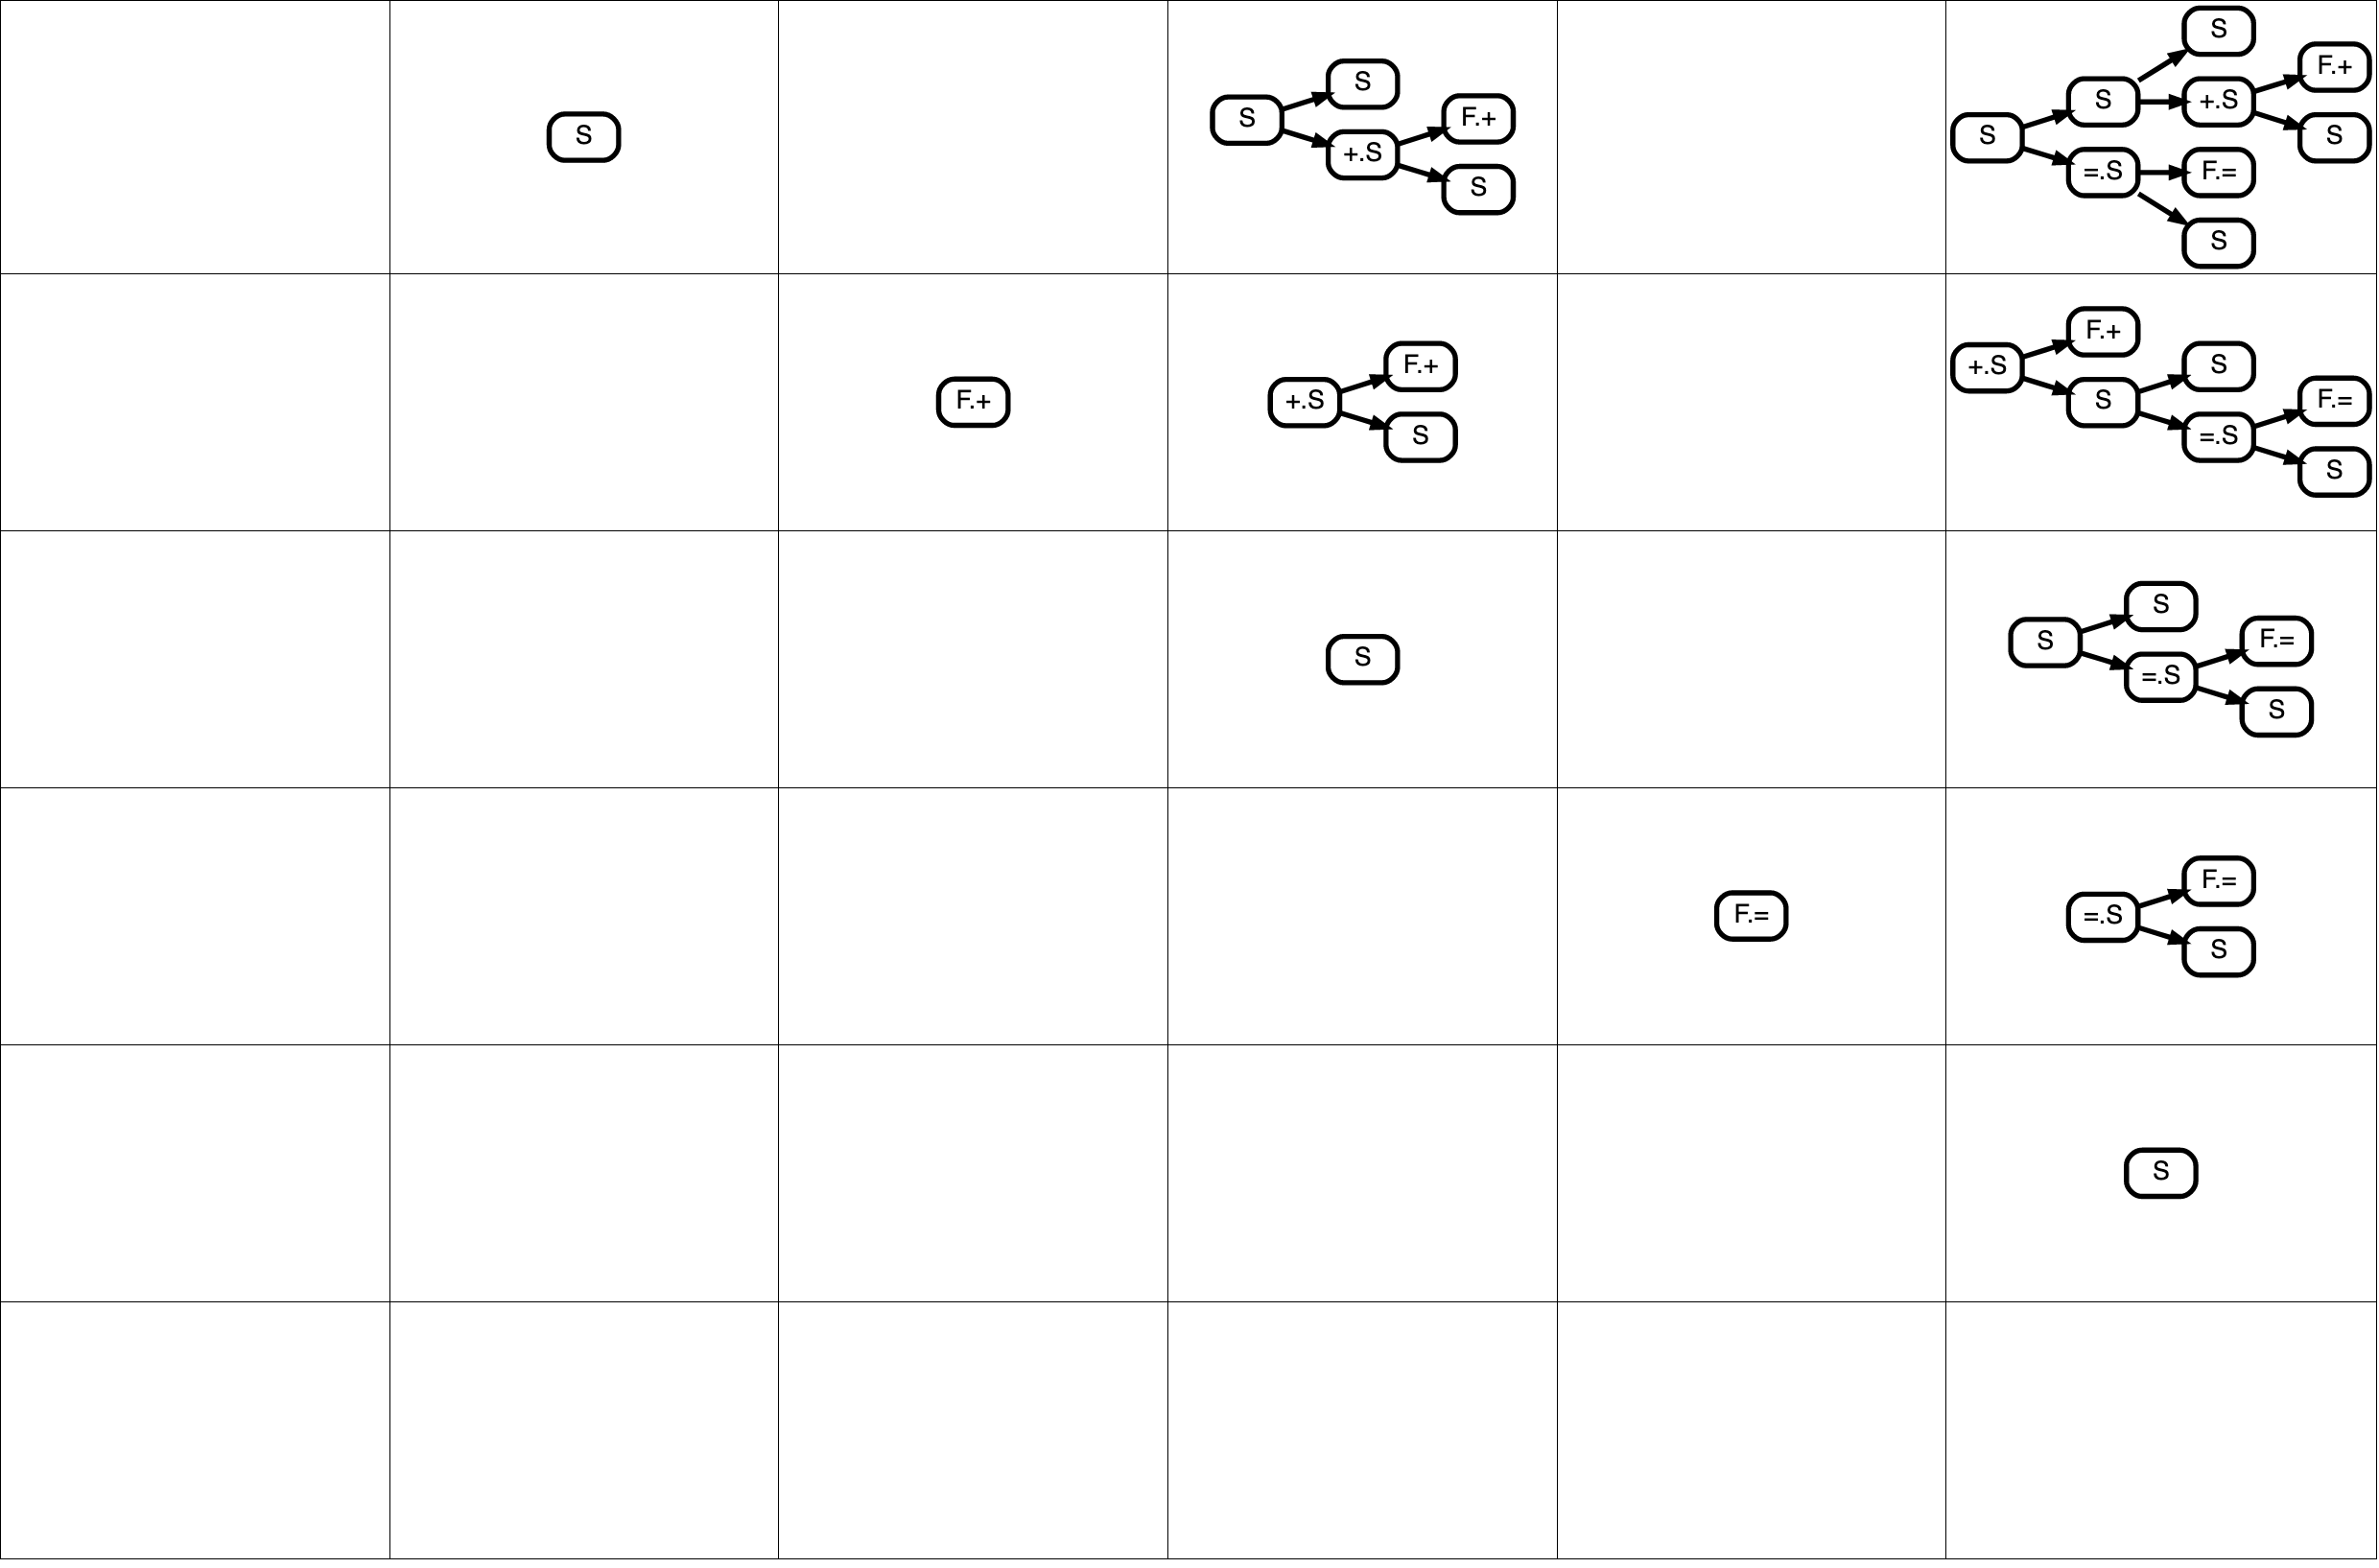
\includegraphics[width=2cm]{../figures/parse4.png}
%%\end{figure}
%
%  \begin{figure}[H]
%    \[
%      \mathcal{M}^* = \begin{pNiceArray}{>{\strut}ccccccc}[margin, extra-margin=2pt,colortbl-like, xdots/line-style=loosely dotted]
%          \vno & \rcr \shup x_1 &  \Cdots      & \mathcal{V}_{1,|x|} & \rcw \mathcal{V}_{1,4} & \cdd & \mathcal{V}^* \\
%          \vdd & \ddd           &  \Ddots      & \rcr\Vdots          & \rcw\vdd               &      & \vdd \\
%               &                &              & \rcr\shup x_{|x|}   & \rcw                   &      & \\
%               &                &              &                     & \mathcal{V}_{4,4}      &      & \\
%               &                &              &                     &                        & \ddd & \\
%               &                &              &                     &                        &      & \mathcal{V}_{n,n} \\
%          \vno & \cdd           &              &                     &                        &      & \vno
%      \end{pNiceArray}
%    \]
%  \end{figure}

%We also need the constraint that no two conflicting nonterminals may be active at any given time... TODO: describe uniqueness constraint
%  \noindent Depicted above is a SAT tensor representing \hlgray{$\sigma_1\:\sigma_2\:\sigma_3$}$\:\_\:\ldots\:\_$ where shaded regions demarcate known bitvector literals $\mathcal{L}_{r,c}$ (i.e., representing established nonterminal forests) and unshaded regions correspond to bitvector variables $\mathcal{V}_{r,c}$ (i.e., representing seeded nonterminal forests to be grown). Since $\mathcal{L}_{r,c}$ are fixed, we precompute them outside the SAT solver.

  \subsection{Deriving the hole locations}

  Valiant's procedure defines a bottom-up synthesizer for a string template with known hole locations. Given a string which contains an error, i.e. $\squiggly\sigma: \Sigma^+$ s.t. $S \notin \Lambda^*_{\sigma}$, where should we put the holes in order for the string to parse? We can derive the hole locations by backpropagating Brzozowski's derivative across upper-triangular entries of $\mathcal{M}^*$. This constitutes to a top-down inference procedure, in which, following the tradition of Bird and Meertens, we define the exponential of a forest as a nested datatype called a \textit{taiga}:

  \begin{align*}
    \text{\textbf{data} \textit{Tree} } a &= \varnothing \mid \langle a, \langle\textit{Tree a, Tree a}\rangle\rangle\\
    \text{\textbf{data} \textit{Forest} } a &= \varnothing \mid \langle \{a\}, \{\langle\textit{Forest a,  Forest a}\rangle\}\rangle\\
    \text{\textbf{data} \textit{Taiga} } a &= \varnothing \mid \langle a, [\langle\textit{Taiga (Taiga a)}\rangle^2]\rangle
  \end{align*}

  This is needed because of the doubly-ambiguous nature of tree search: a single string may have a parse forest, and an incomplete string simultanously occupies a superposition of possible parse forests. When we encounter two adjacent parse forests which cannot be joined, we know that either (1) the left derivation must change (2) the right derivation must change or (3) there must be a hole in the middle which joins the two together. When recursing over the state space, we must simultaneously explore all three possibilities.

  \subsection{Context-Sensitive Reachability}

  It is well-known that the family of CFLs is not closed under intersection. For example, consider $\mathcal{L}_\cap := \mathcal{L}(\mathcal{G}_1) \cap \mathcal{L}(\mathcal{G}_1)$:

  \begin{table}[H]
  \begin{tabular}{llll}
    $P_1 := \big\{\;S \rightarrow L R,$ & $L \rightarrow a b \mid a L b,$ & $R \rightarrow c \mid c R\;\big\}$\vspace{5pt}\\
    $P_2 := \big\{\;S \rightarrow L R,$ & $R \rightarrow b c \mid b R c,$ & $L \rightarrow a \mid a L\;\big\}$
  \end{tabular}
  \end{table}

  \noindent Note that $\mathcal{L}_\cap$ generates the language $\big\{\;a^d b^d c^d \mid d > 0\;\big\}$, which according to the pumping lemma is not context free. We can encode $\bigcap_{i=1}^c \mathcal{L}(\mathcal{G}_i)$ as a polygonal prism with upper-triangular matrices adjoined to each rectangular face. More precisely, we intersect all terminals $\Sigma_\cap := \bigcap_{i=1}^c \Sigma_i$, then for each $t_\cap \in \Sigma_\cap$ and CFG, construct an equivalence class $E(t_\cap, \mathcal{G}_i) = \{ w_i \mid (w_i \rightarrow t_\cap) \in P_i\}$ and glue them together:

  % Generated by cfl4_intersection.vox, open with https://voxelator.com/
  \begin{figure}[H]
  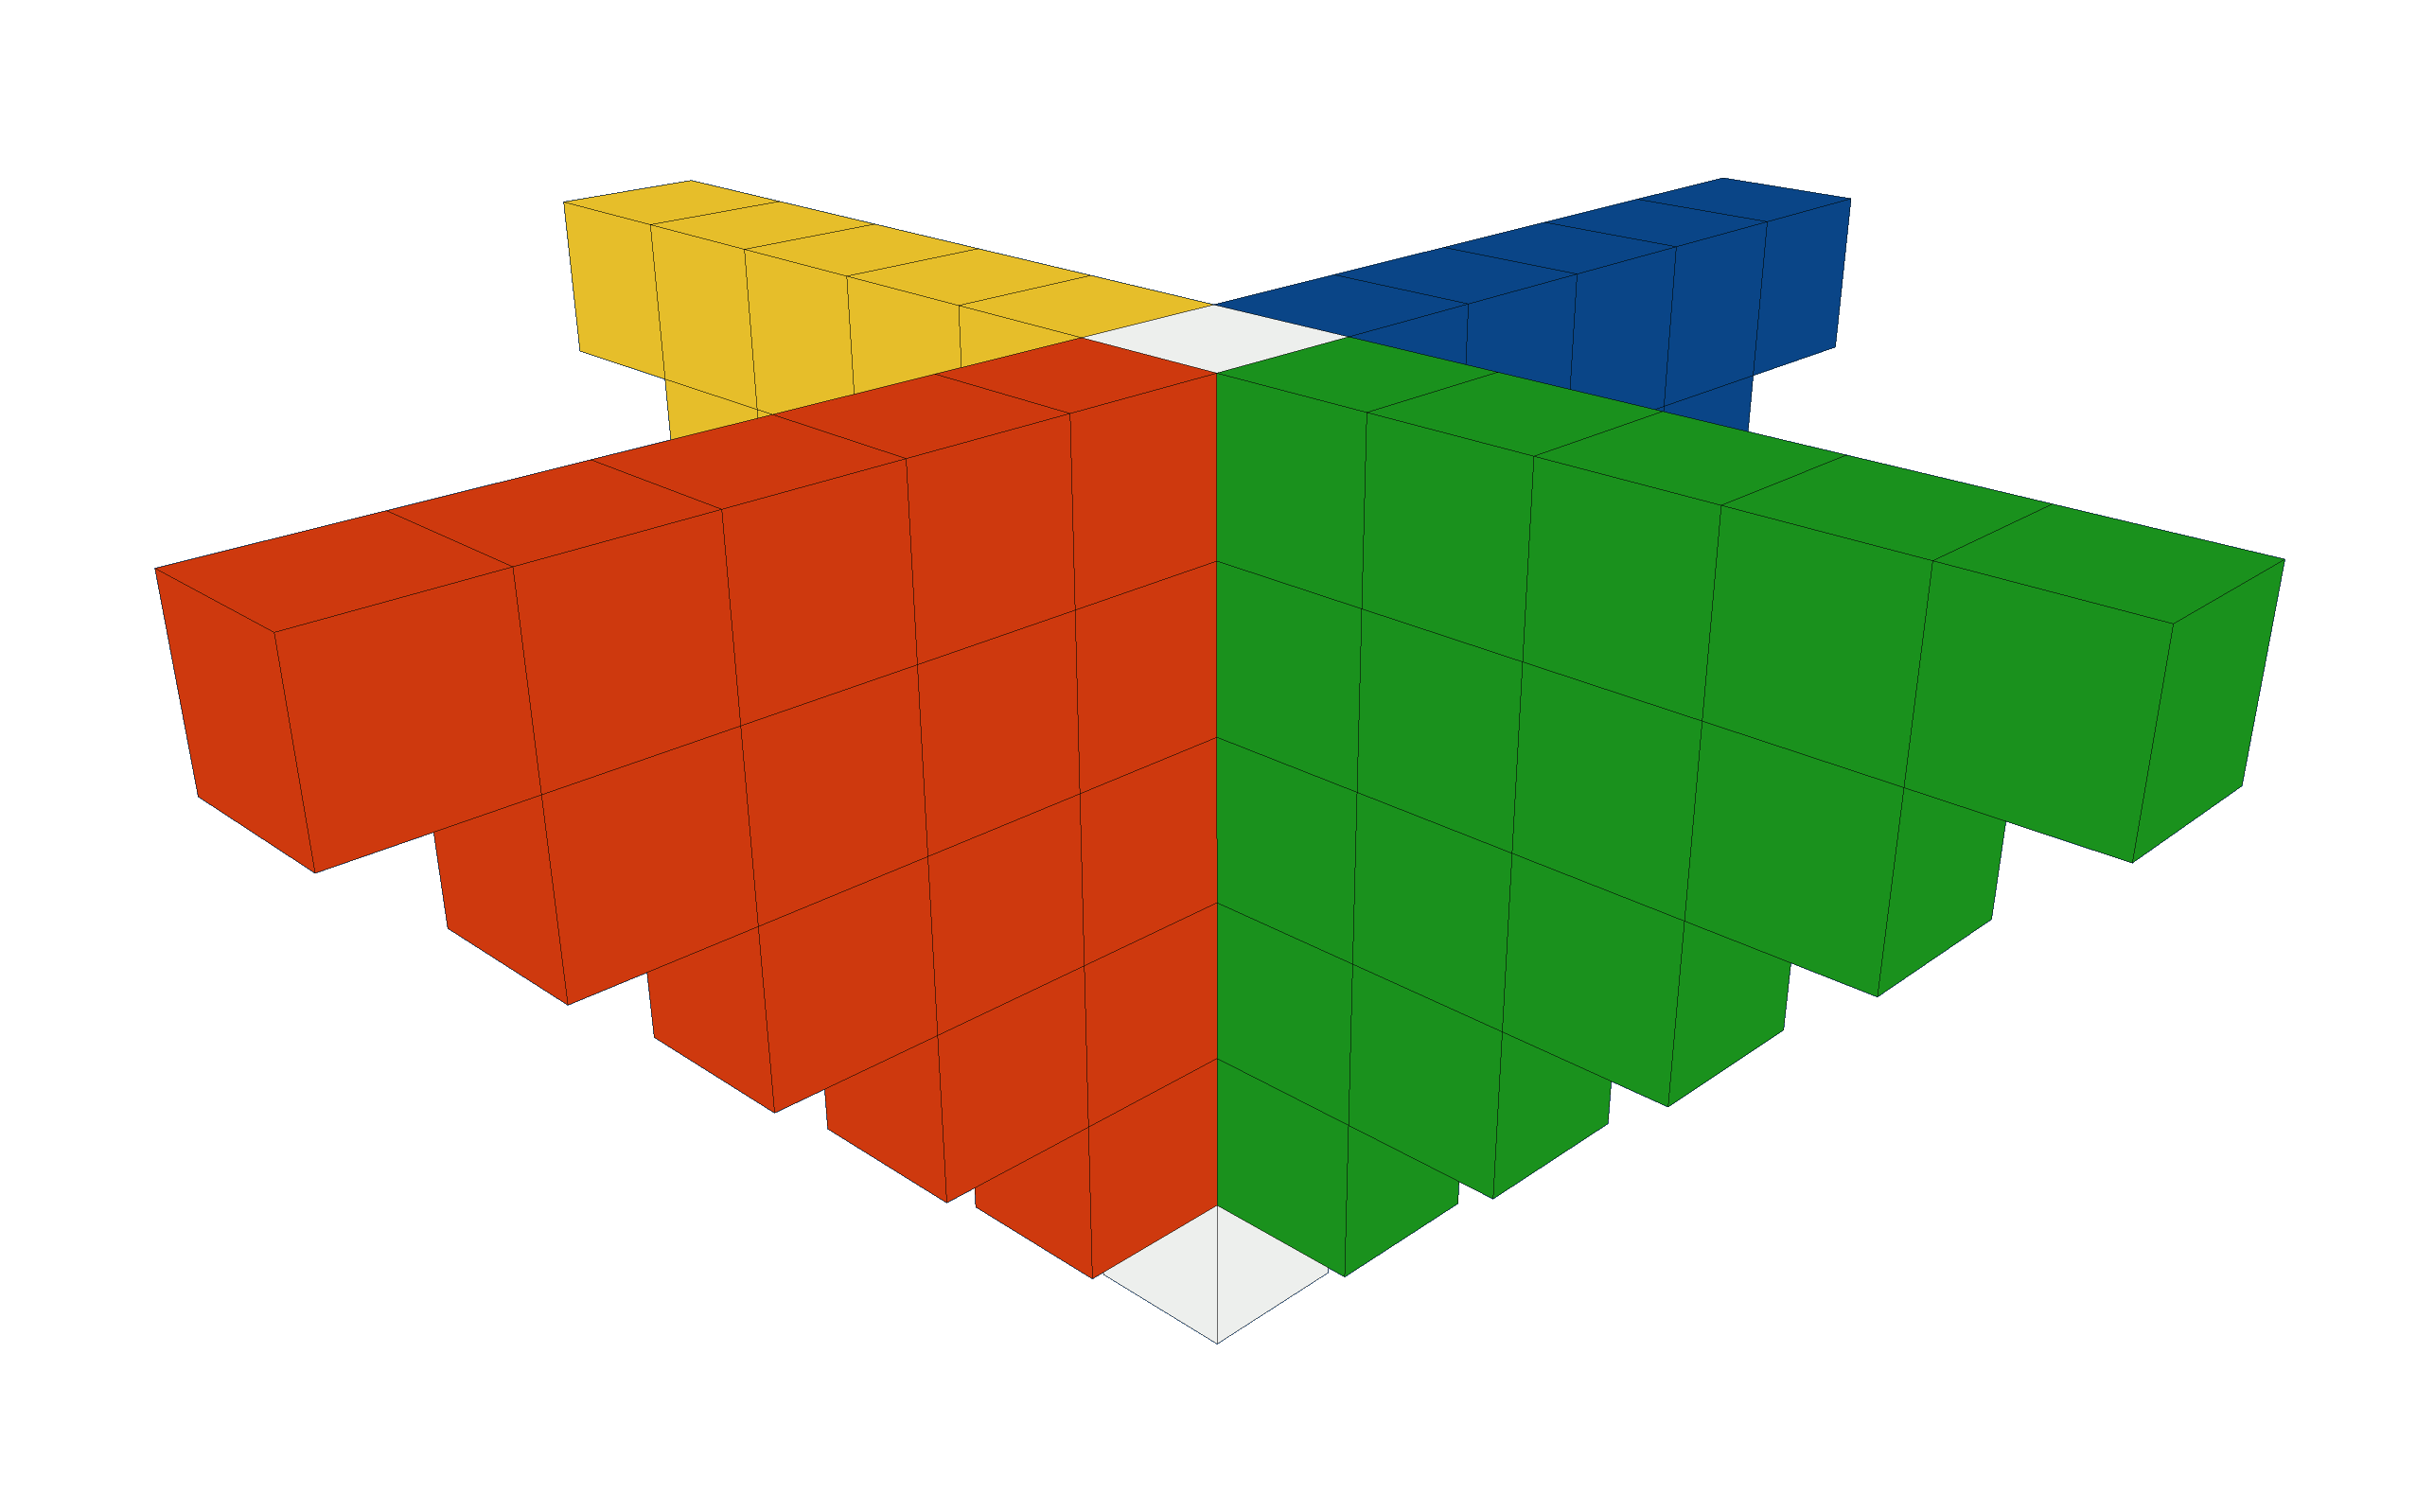
\includegraphics[height=0.063\textwidth]{../figures/angle1.png}\hspace{-5pt}
  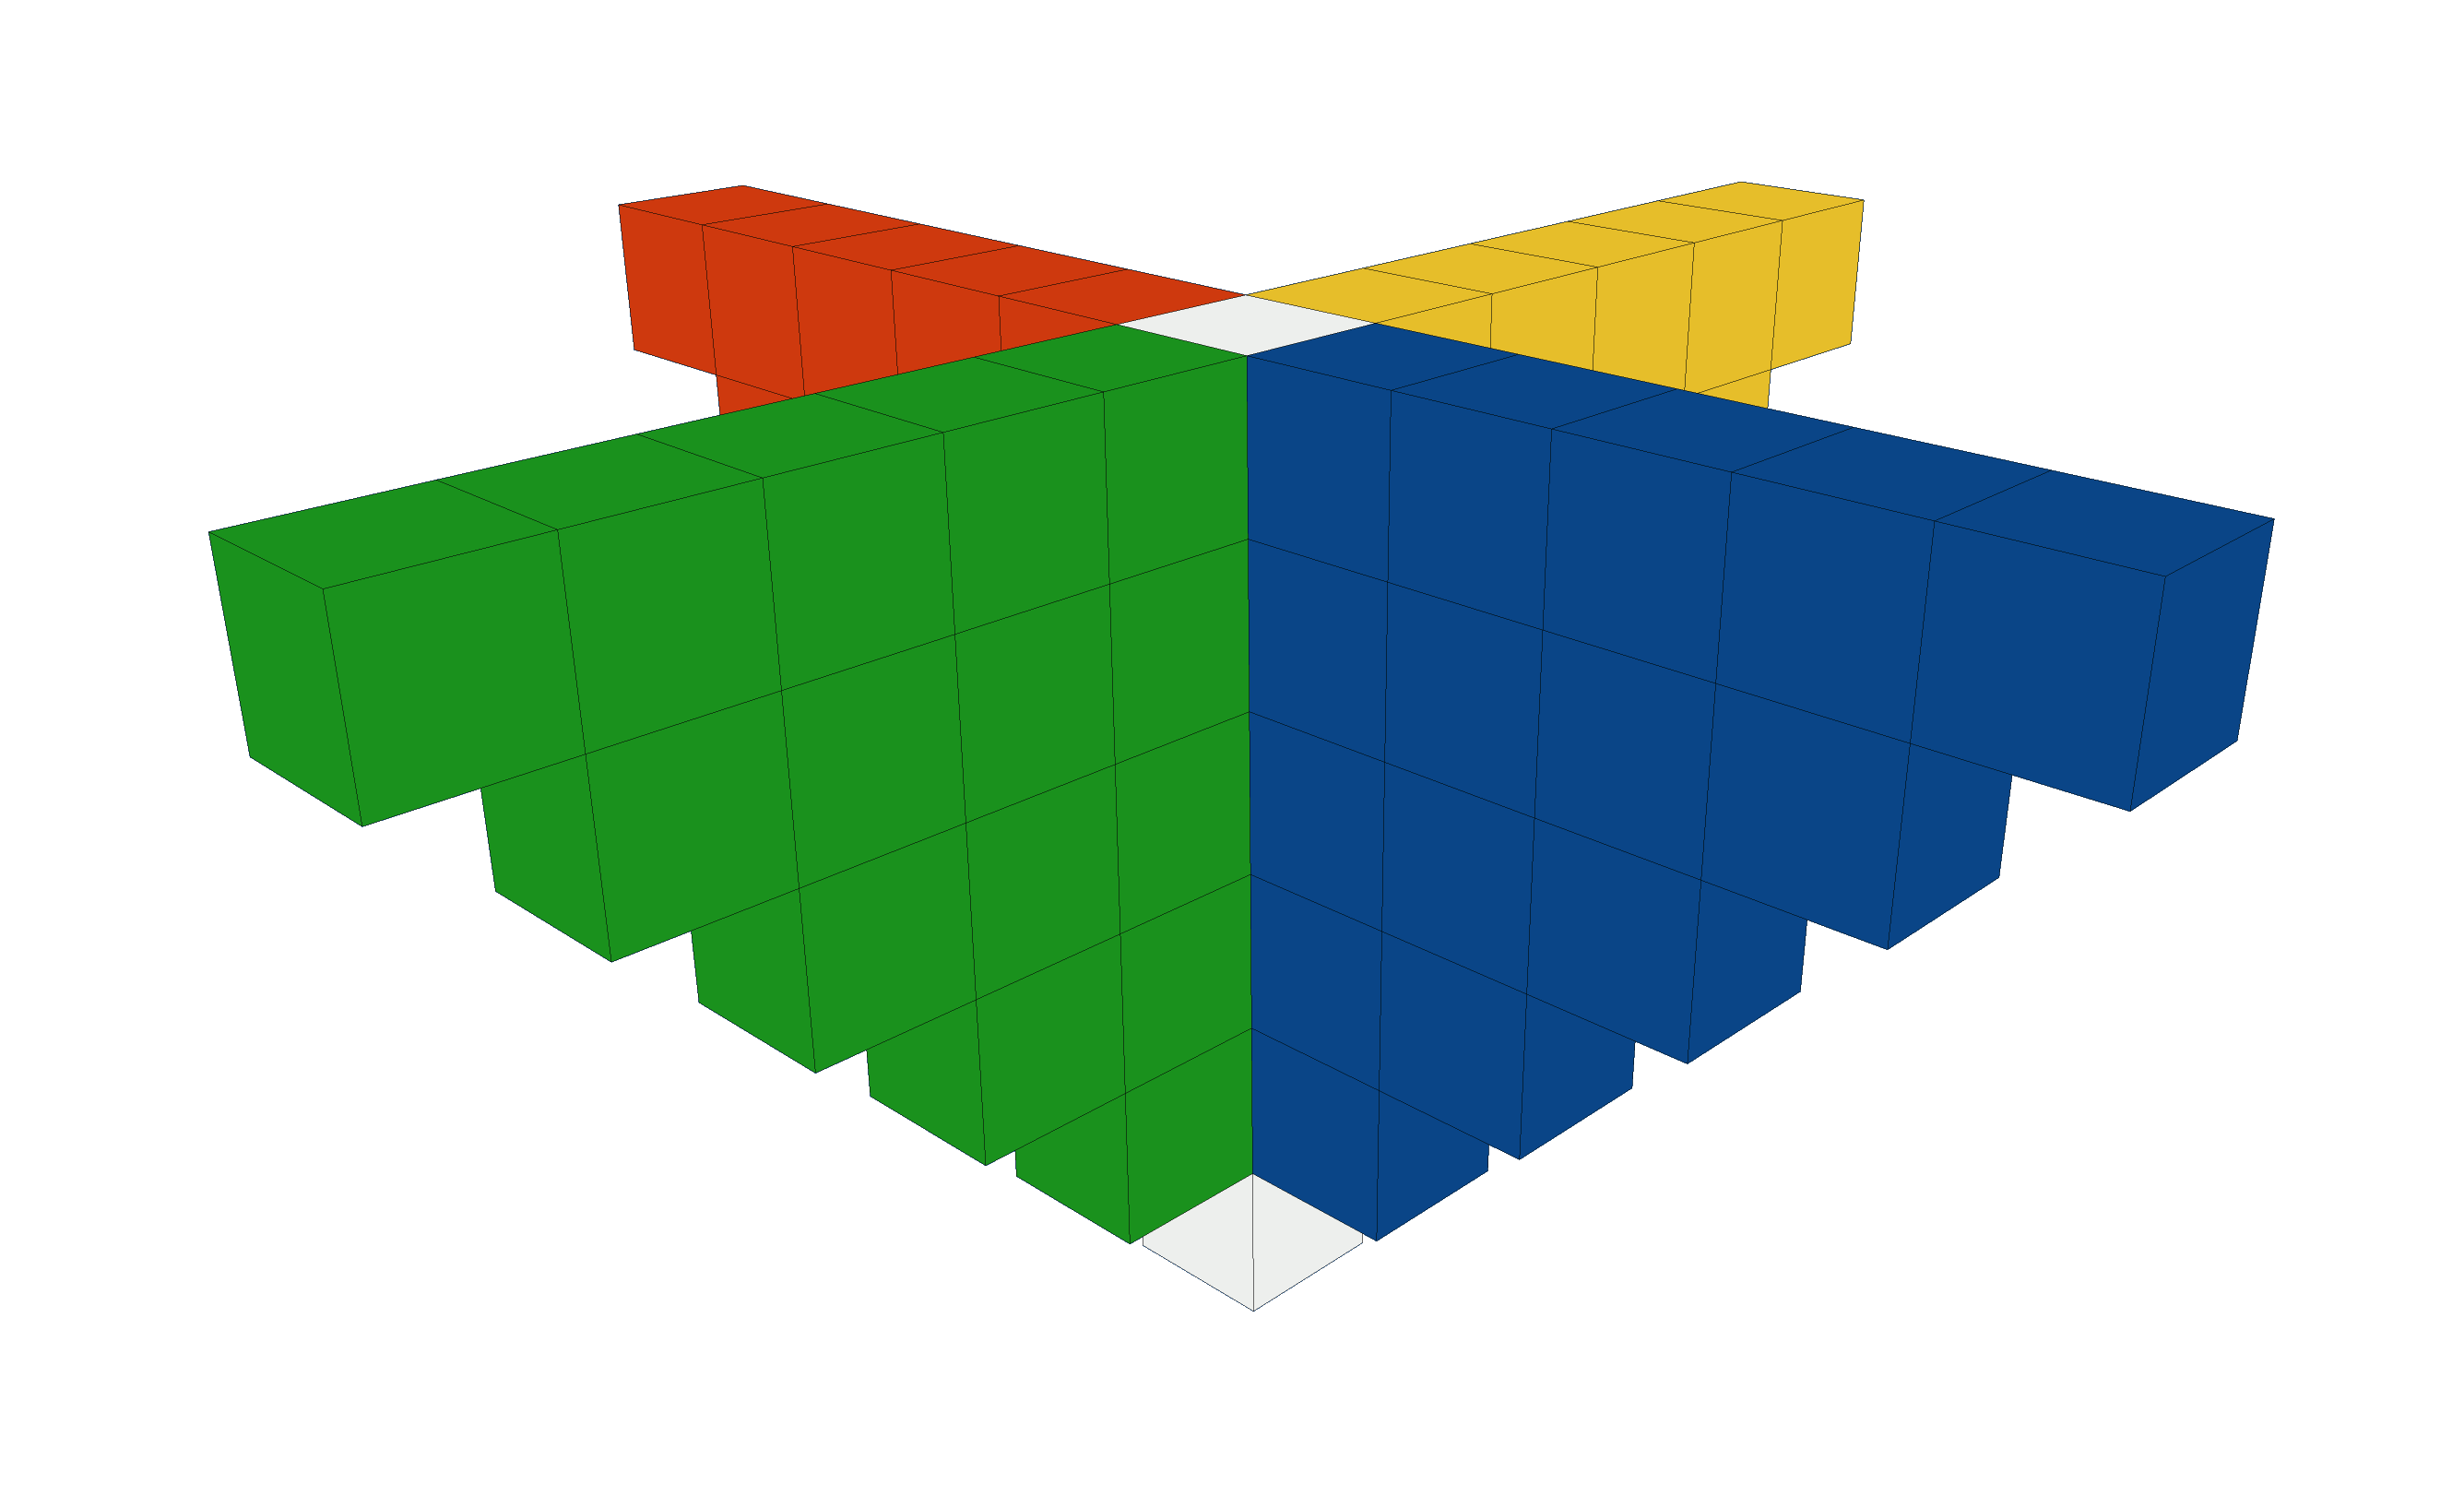
\includegraphics[height=0.063\textwidth]{../figures/angle2.png}\hspace{-5pt}
  
\includegraphics[height=0.063\textwidth]{../figures/angle5.png}\hspace{-5pt}
  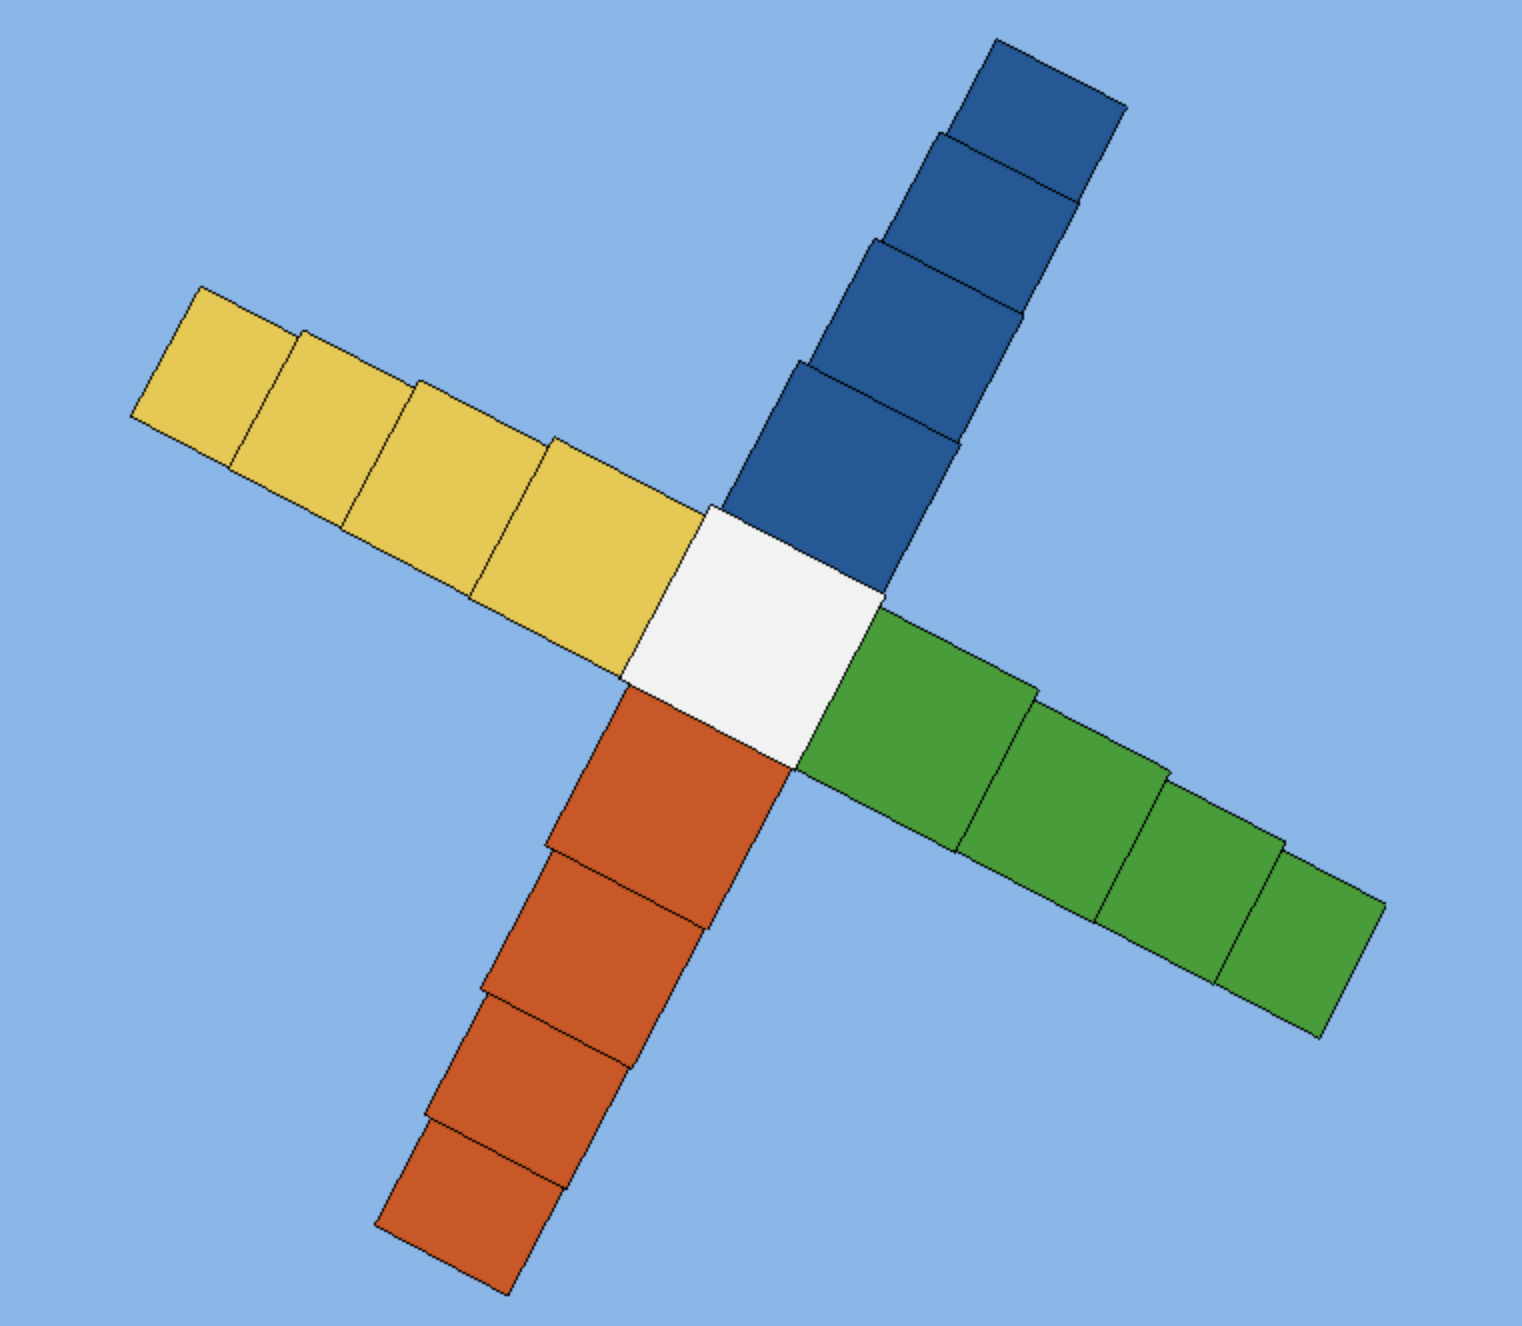
\includegraphics[height=0.063\textwidth]{../figures/angle3.png}\hspace{-3pt}
  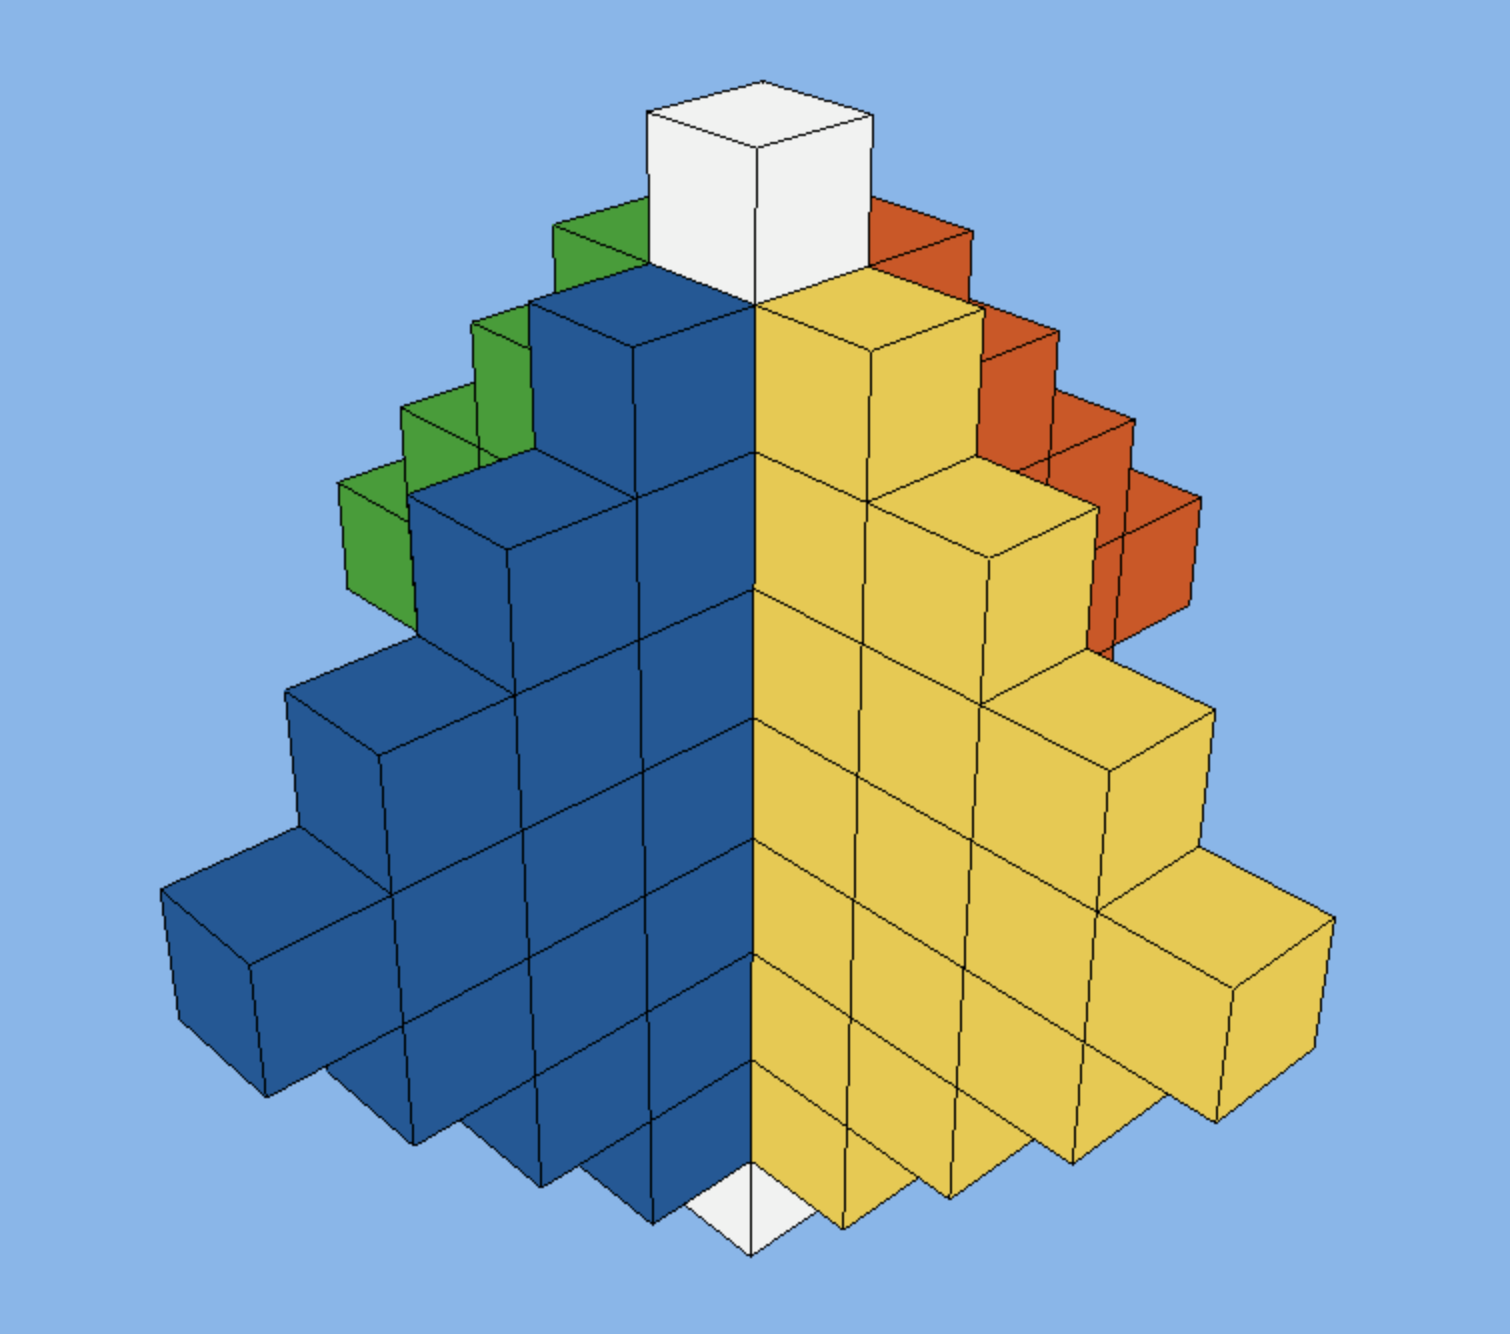
\includegraphics[height=0.063\textwidth]{../figures/angle4.png}
    \caption{Orientations of a $\bigcap_{i = 1}^4 \mathcal{L}(\mathcal{G}_i) \cap \Sigma ^6$ configuration.}
  \end{figure}

  \noindent As $c \rightarrow \infty$, this shape approximates a circular cone whose symmetric axis intersects orthonormal CNF unit productions $w_i \rightarrow t_\cap$, with $S_i \in \Lambda^*_{\sigma}?$ encoded by bitvectors on the base perimeter. Equations of this form are equiexpressive with the family of CSLs realizable by finite CFL intersection.

 \begin{align}
  \bigwedge_{t\in\Sigma_\cap}\bigwedge_{j = 1}^{c-1}\bigwedge_{i=1}^{|\sigma|} E(t_{\cap}, \mathcal{G}_j) \equiv_{\sigma_i} E(t, \mathcal{G}_{j+1})
  \end{align}

%  Together with the uniqueness constraint this ensures that at least one representative of each equivalence class is included... (TODO).

  Although emptiness for CSLs is, in general, undecidable, unsatisfiability corresponds to emptiness of bounded CSLs. Anyhow, since we are working with bounded-width CSLs, everything collapses down to finite languages, which are always closed. Thus, Bar-Hillel and other elegant constructions become trivial when so restricted. So we can use it to decide impossible substrings and other decision problems which are typically intractable in more general settings.

  \section{Conclusion}

  This technique can be used to repair syntax errors in programming languages. It also has the nice advantage that it can provide partial parse trees for invalid strings, i.e., we can decode the tree from the structure of M directly without any special error recovery.

%  \subsection{Deletion, substitution, and insertion}\label{sec:dsi}
%
%  Deletion, substitution and insertion can be simulated by adding a left- and right- $\varepsilon$ production to each unit production:\vspace{5pt}
%
%  \begin{prooftree}
%    \AxiomC{$\Gamma \vdash \varepsilon \in \Sigma$}
%    \RightLabel{$\varepsilon\textsc{-dup}$}
%    \UnaryInfC{$\Gamma \vdash (\varepsilon^+ \rightarrow \varepsilon \mid \varepsilon^+\:\varepsilon^+) \in P$}
%  \end{prooftree}
%
%  \begin{prooftree}
%    \AxiomC{$\Gamma \vdash (A \rightarrow B) \in P$}
%    \RightLabel{$\varepsilon^+\textsc{-int}$}
%    \UnaryInfC{$\Gamma \vdash (A \rightarrow B\:\varepsilon^+ \mid \varepsilon^+\:B \mid B) \in P$}
%  \end{prooftree}
%
%  \vspace{5pt}
%  \noindent To generate the sketch templates, we substitute two holes at an index-to-be-repaired, $H(\sigma, i) = \sigma_{1\ldots i-1}\:\texttt{\_ \_}\:\sigma_{i+1\ldots n}$, then invoke the SAT solver. Five outcomes are then possible:
%
%  \begin{align}
%    &\sigma_{1}\ldots\sigma_{i-1}\:\text{\hlred{$\gamma_1$}\hlred{$\gamma_2$}}\:\sigma_{i+1}\ldots\sigma_{n}, \gamma_{1, 2} = \varepsilon\label{eq:del}\\
%    &\sigma_{1}\ldots \sigma_{i-1}\:\text{\hlorange{$\gamma_1$}\hlred{$\gamma_2$}}\:\sigma_{i+1}\ldots \sigma_{n}, \gamma_1 \neq \sigma_i, \gamma_2 = \varepsilon\label{eq:sub1}\\
%    &\sigma_{1}\ldots \sigma_{i-1}\:\text{\hlred{$\gamma_1$}\hlorange{$\gamma_2$}}\:\sigma_{i+1}\ldots \sigma_{n}, \gamma_1 = \varepsilon, \gamma_2 \neq \sigma_i\label{eq:sub2}\\
%    &\sigma_{1}\ldots\sigma_{i-1}\: \text{\hlorange{$\gamma_1$}\hlgreen{$\gamma_2$}}\:\sigma_{i+1}\ldots\sigma_{n}, \gamma_1 = \sigma_i, \gamma_2 \neq \varepsilon\label{eq:ins1}\\
%    &\sigma_{1}\ldots\sigma_{i-1}\: \text{\hlgreen{$\gamma_1$}\hlorange{$\gamma_2$}}\:\sigma_{i+1}\ldots\sigma_{n}, \gamma_1 \notin \{\varepsilon, \sigma_i\}, \gamma_2 = \sigma_i\label{eq:ins2}
%  \end{align}
%
%  \noindent Eq.~(\ref{eq:del}) corresponds to deletion, Eqs.~(\ref{eq:sub1},~\ref{eq:sub2}) correspond to substitution, and Eqs.~(\ref{eq:ins1},~\ref{eq:ins2}) correspond to insertion. The solutions returned by the SAT solver will be strictly equivalent to handling each edit operation as separate cases.

  \bibliography{../bib/acmart}
\end{document}